\documentclass[a4paper,11pt]{article}
\usepackage{amsmath,amsfonts,amsthm,amssymb,amscd}
\usepackage[top=1in, bottom=1in, left=1in, right=1in] {geometry}
%\pagestyle{headings}

\usepackage[numbers]{natbib}
\usepackage{enumitem}
\usepackage{setspace}
\usepackage{courier}
\usepackage{subcaption}

\usepackage{longtable}

%For inserting sequences of images
%\usepackage{python}
\usepackage{verbatim}
\makeatletter
\newwrite\Code@out

\newcommand\python{\obeylines\expandafter\pythonArg\noexpand}

\newcommand\pythonArg[1][tmp.py.in]{%
    \gdef\FNameIn{#1}
    \gdef\FNameOut{tmp.py.out}
    \begingroup
        \@bsphack%
        \immediate\openout\Code@out\FNameIn%
        \let\do\@makeother\dospecials%
        \catcode`\^^M\active%
        \def\verbatim@processline{%
            \immediate\write\Code@out{\the\verbatim@line}}%
        \verbatim@start}

\def\endpython{%
        \immediate\closeout\Code@out\@esphack
    \endgroup

     %Execute python script. Python directory must be in PATH.
     \immediate\write18{python \FNameIn > \FNameOut}
     \input{\FNameOut}
}

\makeatother

%For increasing the space allowed for floats
\renewcommand\floatpagefraction{0.9}

\usepackage[titletoc, title]{appendix}
\renewcommand{\appendix}{%
  \par
  \setcounter{section}{0}%
  \renewcommand{\thesection}{\thechapter.\Alph{section}}%
}

%graphicx
\usepackage{graphicx}
\graphicspath{{../figures/}}

%endfloat, for placing figures at the end
\usepackage[nomarkers,nofiglist,fighead]{endfloat}
\renewcommand{\efloatseparator}{\mbox{}}

% line spacing
\onehalfspacing

% tab spacing
\newcommand{\tab}[1]{\hspace{.2\textwidth}\rlap{#1}}


% START OF DOCUMENT
\begin{document}
\pagenumbering{roman}

\begin{flushleft}
{\Large
\textbf\newline{Experiments in Natural Network Degradation}
}
\newline
\\
Tony Liu,
Duane A. Bailey

\end{flushleft}



\section*{Abstract}

Dynamic, spatially-oriented systems found in nature such as plant cell arrays or ant colonies can produce complex behavior without centralized coordination or control. Instead, they communicate locally, with these local interactions producing emergent behavior globally across the entire system. The essence of these decentralized systems can be captured utilizing cellular automata (CA) modeling, and such models are utilized for investigating and simulating such natural systems. However, CA models assume spatial regularity and structure, which are certainly not present in natural systems. In fact, natural systems are inherently robust to spatial irregularities and environmental noise. In this work, we relax the assumption of spatial regularity when considering cellular automata in order to investigate the conditions in which complex behavior can emerge in noisy, irregular natural systems.

\newpage

\tableofcontents
\listoffigures

\newpage
\pagenumbering{arabic}
\section{Introduction}
\label{sec:Intro}
Dynamic natural systems have the ability to perform complex tasks that resemble computation, often without the aid of a central processing unit. In particular, spatial systems that are only locally connected, such as plant cell arrays or single-agent populations, can produce emergent, globally-coordinated behavior~\cite{bi07, mo07}. These systems are of particular interest because of their massive parallelism and fault tolerance within noisy, imperfect environments~\cite{si99}. Decentralized dynamic systems can be described and modeled using cellular automata (CA) because of a CA's ability to support complex behavior arising from simple components and strictly local connectivity~\cite{mi96}. The goal with CA models is to able to examine how and under what conditions global, distributed computation emerges in such systems.

One of the main motivating examples of emergent natural computation we have been examining is plant cell stomatal coordination. These dynamic pores control gas exchange within the plant and ``solve'' a constrained optimization problem without a central communication system. What is remarkable about stomata is that their behavior is statistically indistinguishable from the behavior of CAs that solve the \textit{majority problem}: a global coordination task where all cells in the CA need to converge to the majority state of the initial  configuration~\cite{mo07,pe04, we11}. Furthermore, the corresponding majority task automata have been shown to respond robustly in the face of variations in their environment such as state noise, much like their biological counterparts~\cite{me07}. This relationship is exciting because it has been shown that computation in CAs can only occur under specific conditions, existing at a \textit{critical point} between ordered and chaotic behavior~\cite{la90, wf86}. Thus, perhaps we could begin to understand how computation emerges in nature given their established connection with CAs. However, the automata models built to study natural systems like plant stomata make a potentially limiting assumption: regularity of both the cellular grid and the local connections. Dynamic systems in nature certainly do not appear in a uniformly connected lattice. Like their surrounding environment, the spatial orientation of these systems are noisy and prone to irregularities. While some work investigates the effects of nonuniform grids such as Voronoi diagrams or Penrose tilings on automata performance~\cite{ca06,fl01,hi05}, further study is needed to ensure that our models of computation can safely be ``mapped'' to the systems occurring in nature.

With these considerations in mind, this work pursues a deeper exploration of irregular computing CAs. Here, we conduct a series of experiments on a spectrum of automata with irregular grids and connectivities, quantifying their behavior and comparing them to traditional CAs. As noted earlier, computation appears to emerge at a point of criticality somewhere in between the ordered and chaotic automata and \citeauthor{la90}'s $\lambda$ parameter, representing the relative order of a CA, is used to parametrize the possible automata space~\cite{la90}. The $\lambda$ parameter is important because it is an indicator of the class of CAs that have the ability to compute~\cite{wo90}. However, this measure is tuned specifically for static neighborhood definitions and uniform grids. With the experimentation on irregular automata, the goal is to explore and develop a more general notion of $\lambda$ and other metrics so that we can better understand and perhaps even quantify the conditions in which computation can emerge in noisy systems. Another important question we address with this work is whether there is a \textit{qualitative} difference between regular and irregular grid patterns and connectivities: are there cases where uniform CA models are sufficient for representing biological systems? 
% As materiality is also a characteristic of natural systems that typical automata models neglect~\cite{hu07}, we plan on conducting experiments on material-constrained CAs as well. 

We believe that the study of CA behavior in irregular environments is critical to achieve a greater understanding of how biological systems combat imperfections. Ultimately, the contribution of our work on natural computational systems is twofold: not only can we achieve a better understanding of how some biological processes operate, but our knowledge of how these systems work can inspire alternative computing methods~\cite{ma96, si04}. The hope is to illuminate how nature is able to perform complex computation in noisy environments and apply these lessons to advance robust computing models.

\section{Background and Related Work}
\label{sec:Back}

%Why are we interested in distributed computational CA systems? The goal is to achieve a better understanding of how computation naturally emerges from such systems in order to accurately model biological distributed processes as well as improve our technological computing models. We will begin with some motivating examples by considering previous work on applications of robust, distributed CA models, spanning topics such as plant biology, population dynamics, geographic modeling, and computer architecture. However, in order to effectively apply CA models of natural systems, we must understand what computation means in such dynamic systems. Are there requisite properties of computation and if so, how do they arise? For this we consider a collection of papers that develop a framework for quantifying computational characteristics as well as present a hypothesis that computation emerges at the ``edge of chaos.'' Next, as we need to understand how natural computation is robust in the face of noisy and irregular environments, we will examine work on noise and fault tolerance in distributed automata systems. Finally, spatial irregularity is a prevalent feature in nature that is often overlooked in such studies, so we consider some work that examines the impact of such irregularity on dynamic CA systems.

\subsection{Robust Natural Dynamics: Plant Stomatal Patchiness}
\label{subsec:Stoma}
An important motivating example for this work is the modeling of plant cell stomatal coordination done by \citeauthor{pe04}~\cite{pe04}. Plant stomata are dynamic pores distributed across leaves that control gas exchange by opening and closing their apertures. These stomata are solving a constrained optimization problem: they maximize the uptake of CO$_\text{2}$ while minimizing water vapor loss~\cite{mo07,we11}. Long believed to be autonomous units that respond similarly but independently to environmental conditions, it has now been shown that a stoma's aperture is also dependent on interactions with neighboring stomata, sometimes producing coordinated behavior called \textit{stomatal patchiness}, where large groups of stomata uniformly open or close~\cite{pe04}. This phenomenon is poorly understood by biologists, due its highly variable behavior.



%The corresponding majority task CAs have been shown to respond robustly in the face of state noise, imperfect information transfer, and transition rule heterogeneity. In fact, task performance seems to be enhanced in some cases by the presence of noise~\cite{me07}.

\begin{figure}[htp]
	\centering
	\includegraphics[width=1.0\textwidth]{mo07_fig3_maj_task.png}
	\caption[Majority Task CA]{
	An illustration of a majority task cellular automata correctly classifying the majority initial state by converging to black. Figure from \citeauthor{mo07}~\cite{mo07}.
	}
	\label{fig:maj_task}
\end{figure}

\begin{figure}[htp]
	\centering
	\includegraphics[width=0.75\textwidth]{me07_fig3_ca_stoma_comparison.png}
	\caption[Qualitative CA-Stomata Comparison]{
	The left image illustrates coherent state patchiness in a majority task cellular automata. The right image illustrates a similar patchiness for stomata in the plant \textit{Xanthium strumarium L}. Figure from \citeauthor{me07}~\cite{me07}.
	}
	\label{fig:ca_stoma}
\end{figure}

%It is important to note however, that none of these systems are guaranteed to optimally solve the majority task, and even determining whether or not a single instance will perform optimally is hard. The inherent difficulty of determining the success or failure of a given task-performing network emphasizes the importance of information granularity: in an appeal to the concept of self-organizing criticality~\cite{ba88}, small pieces of fine grain information about initial configurations may lend more insight to the global behavior of a distributed network than large but coarse bodies of information about the structure of the space. Thus, studying stomatal patchiness not only provides a step towards connecting computation to phenomenon in nature but also illustrates the central ideas of robustness and criticality.


However, with biological evidence that plant stomata interact locally~\cite{pe04}, task-performing cellular automata are suitable candidates for modelling patchy stomatal conductance. In fact, modeling has shown that the stomatal systems are statistically indistinguishable from CAs configured to solve the \textit{majority task} or \textit{consensus problem}, which involves determining which binary state is the majority state in the initial configuration and then converging all cells to that state (Figure \ref{fig:maj_task})~\cite{gr15}. Qualitative comparisons yield similarities to these task-performing automata as well (Figure \ref{fig:ca_stoma}). The patchiness observed in the plant stomata are analogous to ``transient'' periods that are essential for the computation of majority in CAs. What is remarkable about these stomatal systems is their response to irregularity, as they must manage highly variable and imperfect environments. Though stomatal systems behave similarly to majority task CAs, they face a number of irregularities not accounted for in the CA models such as \textit{heterogeneous interactions}, where local interactions may not be uniform due to stomatal size, orientation, and spacing,  or \textit{modularity}, where leaf veins cause stomata to be subdivided into modules that interact at a level beyond individual interactions~\cite{me07}. Additionally, the stomatal systems must handle temporal \textit{state noise}, where there is natural variability and imprecision in stomatal functioning across time. Thus, \citeauthor{me07} examine the behavior and performance of stomatal-inspired majority task CAs in environments designed to mimic the irregularities with which plant stomata have to contend.

When considering the majority task, most initial configurations are relatively easy for CAs to classify correctly, where there are a large proportion of either ON or OFF cells present in the space. One might expect that the most difficult cases are when the density of ON and OFF cells are roughly equivalent. \citeauthor{me07} note that these hard cases often cause patchiness and are solved correctly only when the patches travel coherently across the CA space, emphasizing the importance of information transfer when supporting task performance in these locally connected networks. Unsuccessful CAs often have ``stubborn'' patches that resist reaching a consensus. Irregularities in the form of heterogeneous interactions, simulated by nonuniform rule tables and random connectivity, and modularity, simulated by grafting together \textit{mosaic networks} of modules, both reduce the performance of the task CAs but do not cripple them~\cite{me07}. In fact, there is evidence that flawed majority task CAs actually \textit{improve} in performance when small amounts of state noise are introduced to the system. \citeauthor{me07} hypothesize that this is because the state noise causes small perturbations in the system, stimulating movement and perhaps freeing previously stubborn patches to move about the state space once more. We have seen how small changes can snowball and sweep through entire the entire CA space; it appears that natural systems also embrace noise and use it to their advantage. Indeed, randomness appears essential in facilitating the self-sustaining and self-informing function of decentralized biological systems.

%\subsection{Foundations of Computation in Dynamical Systems}

%What are the requisite conditions for computation to emerge from a dynamical system? It has been shown that various CA systems can support universal computation~\cite{wf86}, but what are the particular characteristics that allow for computation to be possible? Computational constructs such as Turing machines and other equivalent entities are built upon three fundamentals that can be formulated in the dynamics of a CA system. The system must be able to support the \textit{storage} of information, with the ability to preserve information for arbitrary time periods. Information \textit{transmission} across long distances must also be possible in the environment. Finally, there must be some mechanism for information \textit{interaction} with the potential for information to be transformed or modified~\cite{la90}. These properties are necessary for any dynamical system, automata or otherwise, to have the capacity for computation, but are not sufficient. \citeauthor{la90} also establishes the notion of dynamical systems undergoing ``physical'' phase transitions between highly ordered to highly disordered dynamics, with the most interesting behavior occurring within the boundaries of this transition. This transition region is also where the three requisite properties of computation often occur. Thus, the hypothesis \citeauthor{la90} claims is that computation can spontaneously emerge and dominate the dynamics of a physical system when such a system is at or near such a \textit{critical transition} point~\cite{la90}. 

\subsection{Metrics and Definitions}
\label{subsec:metrics}
\subsubsection*{Cellular Automata}
We will begin with a formal definition of a cellular automaton~\cite{la90}. A CA is composed of a lattice of dimension $D$ with a finite automaton present in each cell of the lattice. There is a finite neighborhood region $\mathcal{N}$, where $N = |\mathcal{N}|$ is the number of cells covered in the neighborhood region. Typical neighborhood stencils for two-dimensions are the five-cell \textit{von Neumann neighborhood} and the nine-cell \textit{Moore neighborhood} (Figure \ref{fig:neighborhoods}). Each cell contains a finite set of cell states $\Sigma$ of size $K = |\Sigma|$ and a transition function $\Delta$ that maps a set of neighborhood configurations to the cell states: $\Delta: \Sigma^N \to \Sigma$. We typically characterize a particular class of cellular automata by the number of neighbors $N$ and the number of cell states $K$. 

\begin{figure}[thp]
\centering
\includegraphics[width=0.75\textwidth]{mi96_fig3_neighborhoods}
\caption[CA Neighborhood Stencils]{
	(a) is the five-cell von Neumann neighborhood, (b) is the nine-cell Moore neighborhood. The gray cell is the one to be updated by a transition rule. Figure from \citeauthor{mi96}~\cite{mi96}.
}
\label{fig:neighborhoods}
\end{figure}

\citeauthor{wf84} proposed a qualitative method for classifying CA automata behavior, with systems falling into one of four classes~\cite{mi96,wf84}:
\begin{itemize}[noitemsep, nolistsep]
\item Class I: All initial configurations relax to the same fixed, homogeneous state.
\item Class II: The CA relaxes to simple periodic structures, perhaps dependent on the initial configuration.
\item Class III: Most initial configurations degenerate to chaotic, unpredictable behavior.
\item Class IV: Some initial configurations result in complex localized structures that have the potential to be long-lived.
\end{itemize}

\subsubsection*{The $\lambda$ Parameter}

The parameter $\lambda$ (Appendix \ref{appA:lambda}) as established by \citeauthor{la90} is used to both narrow the space of CAs to consider as well as to measure the relative homogeneity or heterogeneity of a CA rule table: a completely homogeneous rule table maps all entries to a single \textit{quiescent} state whereas a completely heterogeneous rule table maps entries to random states~\cite{la90}. The parameter is the fraction of the number of non-quiescent mappings in a given rule table, and can be thought of as the average amount of order a given automata transition rule set possesses. Thus, values of $\lambda$ range from $0$, which represents a completely homogeneous rule table to $1 - \frac{1}{K}$, which represents a completely heterogeneous table. There is also a notion of \textit{critical} $\lambda$, denoted $\lambda_c$, where the most complex dynamics tend to emerge. Criticality will be examined in more detail in Section \ref{subsec:edge_chaos}. The hypothesized relationship between $\lambda$ and Wolfram's complexity classes can be seen in Figure \ref{fig:wolfram}.

\begin{figure}[htp]
	\centering
	\includegraphics[width=0.75\textwidth]{la90_fig16_wolfram_classes.png}
	\caption[Wolfram's Complexity Classes]{
	The hypothesized relationship between $\lambda$ and complexity. Class IV CAs would only appear at critical levels of $\lambda$. Figure from \citeauthor{la90}~\cite{la90}.
	}
	\label{fig:wolfram}
\end{figure}

\subsubsection*{Shannon Entropy}

A common quantity used to measure the relative order in a CA system is \textit{Shannon entropy}, denoted by $H$ (Appendix \ref{appA:entrop})~\cite{la90,li90a,wo90}. We can think of Shannon entropy as measuring the amount of information present in the CA space based on the frequency of cell state occurrences; there is less information in ordered systems and more in disordered systems. Thus a completely homogeneous rule table will yield an entropy of $H = 0$ while a completely heterogeneous rule table will yield the maximum entropy possible for that particular $(N,K)$ class of automata. A natural extension to this measure is \textit{mutual information} (Appendix \ref{appA:mut_info}), defined as the correlation between two individual cell entropies~\cite{la90}. We expect some amount of mutual information to be shared across cells in order for computation to be supported: too little shared information degenerates to chaotic behavior, while too much mutual information creates highly correlated structures that are too rigid to support computation.

\subsubsection*{Mean Field Theory}

\textit{Mean field theory}, from the description of many-body systems, in physics is often used to approximate a number of the metrics described above~\cite{li90b,wo90}. The idea is to quantify a many-body system not by considering all mutual two-body interactions (which may become intractable), but rather to describe the interaction of one particle with the the rest of the system by an average potential created by the other particles. This approximation technique is particularly useful when considering classes of automata in the limit, such as in the analysis performed by \citeauthor{wo90}. Approximations for $\lambda$,and $H$ using mean field theory can be found in Appendix \ref{appA:MFT}.

% TODO MFT citation

% TODO Peak statistics (Power Law, etc)

\subsection{The Edge of Chaos: Investigating where Computation Emerges}
\label{subsec:edge_chaos}

It has been shown that various CA systems can support universal computation~\cite{wf86}, but what are the particular characteristics that allow for computation to be possible? Computational constructs such as Turing machines and other equivalent entities are built upon three fundamentals that can be formulated in the dynamics of a CA system. The system must be able to support the \textit{storage} of information, with the ability to preserve information for arbitrary time periods. Information \textit{transmission} across long distances must also be possible in the environment. Finally, there must be some mechanism for information \textit{interaction} with the potential for information to be transformed or modified~\cite{la90}. These properties are necessary for any dynamical system, automata or otherwise, to have the capacity for computation, but are not sufficient. \citeauthor{la90} also establishes the notion of dynamical systems undergoing phase transitions between highly ordered to highly disordered dynamics, with the most interesting behavior occurring within the boundaries of this transition. This transition region is also where the three requisite properties of computation often occur. Thus, the hypothesis \citeauthor{la90} claims is that computation can spontaneously emerge and dominate the dynamics of a physical system when such a system is at or near such a \textit{critical} transition point~\cite{la90}: ``the edge of chaos.'' 

\citeauthor{la90}'s primary method of investigation is a Monte Carlo sampling of two-dimensional CAs, comparing the relationship between the parameter $\lambda$ and the average dynamical behavior of the system, measured by entropy. From both qualitative and quantitative analyses, the most interesting action in two-dimensional CAs occurs in mid-range $\lambda$ values, where the \textit{transient lengths} before static space-time structures emerge is arbitrarily long. Low levels of $\lambda$ have short transient lengths before the CA crystallizes (Figure \ref{fig:order_trans}), and high levels of $\lambda$ have short transient lengths before the CA degenerates into chaos (Figure \ref{fig:chaos_trans}). Levels of $\lambda$ in the middle, however, are a ``sweet spot'' of entropy (Figure \ref{fig:long_trans}). Since information storage involves lowering entropy while transmission involves raising entropy, a balance must be struck in the overall system to support these foundations of computation. Through these experiments and observations, \citeauthor{la90} has established a bound on the complexity of dynamical systems; systems located near the edge of chaos exhibit a range of complex behavior that contain the foundations of computation. Thus, there is a narrow location in the $\lambda$ spectrum of dynamical systems where emergent computation can be discovered, with the maximum complexity occurring at $\lambda_c$ (Figure \ref{fig:lambda_trans}).

\begin{figure}[htp]
\centering
\includegraphics[width=0.5\textwidth]{ordered_transient.png}
\caption[Ordered CA Transient Length]{
The progression of a one-dimensional $N=4$, $K=5$ cellular automaton with $\lambda=0.15$ from a random initial configuration (time progresses from top to bottom). The transient length is short, with the automaton converging to a homogeneous state (all white) within four or five time steps. Figure from \citeauthor{la90} \cite{la90}.
}
\label{fig:order_trans}
\end{figure}

\begin{figure}[htp]
\centering
\includegraphics[width=0.5\textwidth]{chaos_transient.png}
\caption[Chaotic CA Transient Length]{
The progression of a one-dimensional $N=4$, $K=5$ cellular automaton with $\lambda=0.65$ from a random initial configuration. The transient period ends quickly, with dynamic activity degenerating into chaos. Chaotic behavior begins when no cell states can be predicted using information from previously observed states, indicated by the arrow. Figure from \citeauthor{la90} \cite{la90}.
}
\label{fig:chaos_trans}
\end{figure}

\begin{figure}[htp]
\centering
\includegraphics[width=0.20\textwidth]{long_transient.png}
\caption[Complex CA Transient Length]{
The progression of a one-dimensional $N=4$, $K=5$ cellular automaton with $\lambda=0.5$ from a random initial configuration. The transient length is quite long (over 10,000 time steps), indicative of more complex dynamic activity. Figure from \citeauthor{la90} \cite{la90}.
}
\label{fig:long_trans}
\end{figure}

\begin{figure}[htp]
\centering
\includegraphics[width=0.5\textwidth]{la90_fig3_lambda_transient_len.png}
\caption[Lambda and Transient Length]{
Average transient length as a function of $\lambda$ for a 1D CA. The long transient lengths centered around $\lambda_c=0.5$ indicate the transition between ordered and disordered dynamics. Figure from \citeauthor{la90} \cite{la90}.
}
\label{fig:lambda_trans}
\end{figure}

%Work has been done to pinpoint precisely where this transition point occurs, continuing along the parallels between CAs and transitions in physical systems. Utilizing mean field theory, theoretical approximations of the entropy against $\lambda$ in two-dimensional automata made by \citeauthor{wo90} closely match previous experimental results. As the number of total possible cell states approaches infinity, there is a sharp phase transition occurring at $\lambda=0.27$, akin to first-order transitions in actual physical systems~\cite{wo90}. Perhaps this is the critical $\lambda$ point for this particular class of CAs. These results show promise in the parallels between physical systems and the dynamic behavior of cellular automata. However, to investigate this in further detail, it may be necessary to identify other statistical properties in order to fully determine the phase transition point.

%These findings illustrate an important point: statistics that measure the behavior of these CAs may apply an implicit filtering bias on the class of automata, and so structure may be revealed under different measures that is not present under other measures, as shown by $\lambda$'s classification of the optimal CAs for the majority task as chaotic. \citeauthor{la90}'s hypothesis that $\lambda$ correlates with computational ability appears to need refinement: $\lambda$ may very well correlate with the average behavior of CAs but what is the significance of  ``average behavior,''  especially when $\gamma$ is high in the critical regions of interest? For a given $N$ and $K$, CAs that have the potential to compute may reside in a wide range of $\lambda$ values, illustrating the need for a more precise metric. \citeauthor{mi93} also stress that the focus should be harnessing the computation ``naturally'' present within a CA rather than attempting to impose traditional definitions of computation upon them. 

Throughout our exploration of computation in distributed dynamic systems, we often see a delicate balance struck between order and chaos in order to support complex behavior: information must be both propagated (high entropy) and stored (low entropy), and minute alterations in local configurations can have catalytic global effects. What happens when this balance is disturbed? Thus far we have only considered highly regular environments for computation in CA systems, with uniform lattice grids and rule tables. Do these systems behave robustly when the environments are not well-structured? Dynamic natural systems serve as ``the ultimate proof of concept,'' as they are able to function despite residing in environments (the real world) that are inherently noisy and irregular~\cite{si99}. 

\subsection{Aperiodicity: Moving Away from Regular Spatial Representations}

There are some who question the viability of traditional CA models as adequate simulations of real-world phenomenon. Beyond the obvious limitation that real-world systems rarely exist in regular grids, a primary concern is that neighborhood definitions are entirely dependent on the structure of the grid configuration, making it difficult to define alternative neighborhood stencils beyond variations of the standard Moore or von Neumann neighborhoods. The local connectivity can be varied by using different shapes such as hexagons as tiles, but the number of neighbors per cells are still restricted to the same amount across the space. Thus, in order to support richer neighborhood interactions, the size of the neighborhood must be variable while still respecting the local connectivity of the grid. We consider a first step in this direction by examining an alternative formulation of the Game of Life played on aperiodic Penrose Tiles.

The Game of Life, discovered by John Conway, is a $K=2$, $N=9$ two-dimensional cellular automaton that is particularly remarkable because of both the rich emergent structures it can generate as well as its Turing universality~\cite{ga70}. Most instances of the Game of Life are played on regular, two dimensional lattices. What changes in behavior occur when it is simulated on an aperiodic \textit{Penrose} tiling? \citeauthor{hi05} examined this variation, and in particular ran experiments that explored the \textit{lifetimes} (number of generations until stabilization) as well as  \textit{ash densities} (the fraction of ON cells in a stabilized configuration) of random initial configurations. The Game of Life on the Penrose tiles have lifetimes that are much shorter and ash accumulation half as dense as simulations on the regular lattice~\cite{hi05}; this is likely due to the irregularity in the tiling distribution, illustrating that, at least in this instance, the variable neighborhood sizes across the grid make it more difficult to maintain coherent structures.

TODO Penrose Background (Owen and Stepney, Bailey and Lindsey)

\subsection{Summary}
\label{sec:PrevSum} 

We have seen throughout this review that work on the computational dynamics of distributed natural systems is a two-way street, with researchers both utilizing cellular automata to investigate complex behavior in natural systems as well as drawing inspiration from nature to build more robust and efficient ``cellular computers.'' Additionally, there has been extensive work examining how dynamic systems can give rise to computation with an abundance of metrics that can be used to analyze such systems. It would be reasonable to apply the measures from these computational criticality studies to attempt to understand natural systems. Unfortunately, there is not a clear mapping between the foundational structures of cellular automata and dynamical natural systems. Assumptions cannot be made about a potential correspondence between local connections, transition rules, or spatial orientation when CAs and natural systems operate within such contrary environments: the control and precision of computer simulation versus the noise and inconsistency of the real world. There is inherent imprecision when dealing with natural systems, which makes utilizing the criticality statistics problematic. The definitions of metrics like $\lambda$ as well as the notion of average dynamic behavior can be difficult translate to systems where there are no structural uniformities that can serve as a foundation for measurement. We have to adapt these metrics to the domain of irregular cellular automata in order to properly investigate the nature of computation in such systems. 
%\processdelayedfloats

\section{System Design}
\label{sec:System}

\subsection{Architecture Overview}
Our CA simulation platform was designed primarily with flexibility in mind. 
It follows an event-driven architecture written in C++; actions are placed on a queue and are performed one at a time. 
The event queue structure allows us to easily interleave actions in between time steps of a CA simulation; for example, we can take snapshots of the grid state or dump measurements to a file in between time steps at any frequency we wish. 
Modular components and data structures can easily be swapped in and out of the simulation platform, giving us fine-grained control over the experiments we are running. 

Termination of the CA simulation occurs either when a maximum time step is reached, or when a grid state is repeated. 
We track grid states by walking through all cells on a grid in a consistent order, appending each cell state to a string array and then passing the resulting string through a hash function. 
We keep a history of these hashes along with the time step they occur, and terminate the simulation if a hash is ever repeated. 
Recording the time step also allows us to track the periodicity of any potential oscillating structures occurring within the simulation.

We execute rule table updates across the grid in a ``spreading activation'' fashion in order to increase the performance of the simulator. 
Instead of visiting and updating each cell, we track which cells changed state in the previous time step and place those cells along with their neighbors in a \textit{change} list. 
When updating the graph for the next time step, we only apply the transition rule to cells in the list. 
We then repeat this process, updating the list with any cells and their neighbors that have changed state. 
We initialize the change list at the beginning of the simulation to all cells in the grid. 
This method of applying updates allows us to only consider cells that could potentially change, saving time throughout the CA simulation especially if the grid is large. 

\subsection{Grid Generation}
\label{subsec:GridGen}

\subsubsection{Delaunay Triangulations and Voronoi Diagrams}
The goal with building grids using Voronoi diagrams is to produce irregular grids that still respect Euclidean distance, as discussed in Section \ref{subsec:ModelVoronoiRep}. Given a set of \textit{generator points} $\{p_1, ..., p_n\}$ in the plane, a Voronoi polygon $V_k$ corresponding to a generator point $p_k$ consists of all points whose distance to $p_k$ is less than its distance to any other generator point. Thus, we can partition the plane into Voronoi polygons that correspond to every generator point, producing a \textit{Voronoi Diagram}. These polygons will serve as the cells in our CA simulations. 

The first step in the process to generate a Voronoi-based grid is to produce generator points. We use \textit{Poisson Disk Sampling} to generate random points that are guaranteed to be at least some specified distance apart from each other~\cite{br07}. Points created by this method will avoid the clumping that can occur when a random uniform distribution is used, illustrated in Figure \ref{fig:pt_gen}.

\begin{figure}[htp]
\centering
\begin{subfigure}[t]{0.6\textwidth}
  \centering
  \includegraphics[width=\textwidth]{ch3_figs/uniform_cloud_edited}
  \caption{Uniform Distribution}
  \label{fig:penrose_types:kd}
\end{subfigure}

\begin{subfigure}[t]{0.6\textwidth}
  \centering
  \includegraphics[width=\textwidth]{ch3_figs/poisson_cloud_edited}
  \caption{Poisson Disk Sampling}
  \label{fig:penrose_types:tt}
\end{subfigure}

\caption[Random Point Generation]{
  Representative point distributions when utilizing uniform random distribution and Poisson Disk sampling. Notice how points can ``clump'' when using a uniform distribution while points are more evenly spaced when using Poisson Disk Sampling.
}
\label{fig:pt_gen}
\end{figure}

Once we have a set of generator points, we construct the dual graph of the Voronoi Diagram, known as the \textit{Delaunay Triangulation}. The Delaunay Triangulation of a set of points $\{p_1, ..., p_n\}$ in the plane is a triangulation such that no point $p_k$ resides inside the circumcircle of a triangle. We utilize the \textit{Flip Algorithm} to construct the Delaunay Triangulation; though the flip algorithm is not the fastest Delaunay Triangulation algorithm, it is straightforward to implement, requires no auxiliary data structures, and performs well enough for our purposes.

Given a Delaunay Triangulation, we can produce its corresponding Voronoi Diagram by calculating the circumcenter of each Delaunay triangle and creating an edge between the circumcenters of adjacent triangles~\cite{de11,ed08}. The circumcenters of the triangles correspond to Voronoi polygon vertices, so we obtain valid Voronoi regions. Thus we have obtained both the graph representation and the geometric representation of a Voronoi-based grid. An illustration of this process is shown in Figure \ref{fig:voronoi_gen}.

\begin{figure}[htp]
\centering
\begin{subfigure}[t]{0.4\textwidth}
  \centering
  \includegraphics[width=\textwidth]{ch3_figs/stoma_pts_square_edited}
  \caption{Generator Points}
\end{subfigure}
~
\begin{subfigure}[t]{0.4\textwidth}
  \centering
  \includegraphics[width=\textwidth]{ch3_figs/d_stoma_square_edited}
  \caption{Delaunay Triangulation}
\end{subfigure}

\begin{subfigure}[t]{0.4\textwidth}
  \centering
  \includegraphics[width=\textwidth]{ch3_figs/v_stoma_square_edited}
  \caption{Voronoi Diagram}
\end{subfigure}
\caption[Voronoi Diagram Generation]{
	The Voronoi Diagram construction process. We begin with a random set of points (Figure a), compute the Delaunay Triangulation (Figure b), and subsequently the Voronoi Diagram (Figure c).

}
\label{fig:voronoi_gen}
\end{figure}
\subsubsection{Voronoi Quadrilaterals}
\label{subsec:vquad}
Experiments and simulations involving $\lambda$ require static neighborhood sizes across all cells in the grid. One way we address this requirement is by generating irregular grids that have cells of the same number of sides. Specifically, given a Voronoi Diagram we can further partition the region such that all cells in the plane are quadrilaterals. This conversion is accomplished by taking two edge-adjacent Voronoi polygons and forming a quad from the two generator points and the end points of the shared common edge between the polygons (Figure \ref{fig:vquad_gen})~\cite{am10}. As long as the given Voronoi Diagram is well-formed, specifically with all generator points placed at least some minimum radius from each other, this quadrilateral generation is possible across an entire Voronoi diagram, as seen in Figure \ref{fig:vquad_grid}. Note that though cells in the resulting \textit{VQuad} grid always share edges with four other neighboring cells (excluding the boundary) resulting in uniform generalized von Neumann neighborhood sizes across the grid, the number of cells they share vertices with are variable. This variability in vertex adjacency is partially due to the presence of concave quadrilaterals in the resulting grid. %TODO tessellation right here?

\begin{figure}[htp]
\centering
\includegraphics[width=0.75\textwidth]{ch3_figs/vquad_generation}
\caption[Voronoi Quad Generation]{
	An illustration of the Voronoi quadrilateral creation process. Generator points $A$ and $B$ are connected with the shared edge endpoints $1$ and $2$ to create the quadrilateral pictured on the right. Figure adapted from \citeauthor{am10}~\cite{am10}. 
}
\label{fig:vquad_gen}
\end{figure}

\begin{figure}[htp]
\centering
\includegraphics[width=1.0\textwidth]{ch3_figs/vquad_stoma_v2}
\caption[Voronoi Quad Grid]{
  A representative Voronoi Quad grid. Note that most of the cells are convex and all non-boundary cells have four  edge-adjacent neighbors.
}
\label{fig:vquad_grid}
\end{figure}

\subsection{Grid Degeneration}

\subsubsection{Generator Point Removal}
\label{subsec:gen_pt_rem}
As noted in Section \ref{subsec:vquad}, VQuad grid generation is dependent on the position of Voronoi generator points in the input Voronoi diagram. Thus, one simple manner of grid degeneration is to remove generator points from the input diagram. Because a generator point in the input diagram could be a vertex to many VQuad cells, generator point removal has the effect of taking out large chunks of the VQuad grid, as pictured in Figure \ref{fig:genpt_degen}.

\begin{figure}[htp]
\centering
\includegraphics[width=1.0\textwidth]{ch3_figs/gen_pt_degen_7}
\caption[Generator Point Degradation]{
  A VQuad grid degraded by the removal of 7\% of the input generator points. Notice the lack of small, (particularly single cell) holes in the resulting grid.
}
\label{fig:genpt_degen}
\end{figure}

\subsubsection{Crosshatching Degeneration}
\label{subsec:ch_degen}
Though generator point removal provides a simple way to degrade a grid, we wanted finer-grained control over how points and edges are removed. We devised a manner of degradation that allowed us to specify what local regions of the grid would be disconnected from other portions of the grid. This basic premise is to draw vertical and horizontal lines at regular width $w$ intervals apart that subdivide the irregular grid roughly into square lattice regions. Cell edges that intersect these \textit{crosshatchings} are removed from the grid with some probability $p$: cells that were formerly connected by the edge no longer are neighbors in the graph representation of the grid. Thus at $p=1.0$ we would have completely isolated ``islands'' of grid subregions. This \textit{crosshatching degeneration} technique allows us control over the degree of regional connectivity, as pictured in Figure \ref{fig:crosshatch_degen}. This manner of degradation preserves the number of cells present in the grid, instead introducing degradation by decreasing edge adjacency. Though we primarily use crosshatching degeneration as a form of edge removal, this technique also gives us a way to control generator point removal: since the crosshatchings define a square lattice partitioning of the grid, we can also choose square regions to remove with some probability $p$. Any generator points sitting within the boundary of a chosen square region will be removed from the graph. Thus we can control both the frequency of generator points removed (through adjusting $p$) as well as the average size of the of the regions removed (through adjusting $w$). This crosshatching technique allows us to parameterize the degeneration of a grid beyond simply measuring average neighborhood size.

\begin{figure}[htp]
\centering
%TODO add crosshatch degeneration figure
\includegraphics[width=1.0\textwidth]{ch3_figs/ch_p100_w20}
\caption[Crosshatching Degeneration]{
	An illustration of a $p=1.0$, $w=20$ crosshatch degenerated grid: edges marked in red have been removed from the connectivity graph.
}
\label{fig:crosshatch_degen}
\end{figure}

\subsection{$\lambda$ Rule Tables}
\label{subsec:ch3_lamb}
%wolfram command is: rotations with 4 beads, 8 colors
%TODO Burnside's lemma?
In the $\lambda$ experiments performed by \citeauthor{wo90}, rule tables must be \textit{isotropic}: all planar rotations of a particular neighborhood configuration map to the same output cell state. This condition removes the global property of spatial orientation from influencing rule transitions~\cite{av00,wo90}. As a result, what would be a $K^N$ sized table results in a smaller table because only rotationally distinct neighborhood configurations are unique entries. To generate these tables, we iterate over all $K^N$ possible neighborhood values, canonicalize their string representations by finding their \textit{lexicographically minimal rotation}, and track only the unique neighborhoods. For example, in the $K=8, N=5$ case, neighborhoods ``0110'' and ``1001'' map to the same minimal rotation neighborhood of ``0011''. We then append a center state value to the end of this canonical neighborhood representation, thus creating the keys for our $\lambda$ rule table mapping with the output state for that particular neighborhood configuration as the value.

Rule tables must also be \textit{strongly quiescent} in that a neighborhood configuration that consists entirely of the quiescent state must map to the quiescent state. This condition is satisfied by initializing the appropriate entry in the transition table and then ensuring that entry is not modified throughout a given experiment run.

%\processdelayedfloats

\section{Local Majority Experiments}
\label{sec:local_maj}

As discussed in \ref{sec:Back}, \citeauthor{me07} investigated CA performance on the majority task in the presence of various irregularities, such as temporal state noise, nonuniform rule tables and random connectivity in an exploration of robustness in stomatal dynamic systems. We extend this work by examining the effects of spatial irregularity on CA majority task performance.

\subsection{Baseline Majority Task Performance on Irregular Grids}

Our extensions of majority task experiments will focus on the \textit{local majority} rule table for 2-state cellular automata. The rules are simple:

\begin{itemize}
\item If there is a majority of ON or OFF cells in a cell $c$'s neighborhood, then $c$ will transition to the majority state, and
\item If there is no majority, $c$ will retain its previous state.
\end{itemize}

\noindent This rule table represents the most basic manner of solving the majority task and is easily extended to grids with variable neighborhood sizes.

\subsubsection*{Experimental Setup}
We mirror \citeauthor{me07}'s experimental setup in order to compare our results with theirs. For regular grids, a 15 by 15 grid (225 total cells) is utilized with periodic boundaries. We begin with a 1:99 ON:OFF ratio, incrementing by 1 up to 99:1. The simulation is run for a maximum of 450 time steps, recording only completely correct classification. 1,000 random grid configurations are used for every starting ratio, giving a total of 99,000 trials. A single complete run of all the trials takes approximately 25 minutes in our simulation system.

We use Delaunay and Voronoi generation methods to generate our irregular grids. Our experiments utilize both a grid created through Poisson Disk generator points (Figure~\ref{fig:lm_delaunay}) as well as a grid derived from a plant stomatal array. For the stomatal array, we begin with an image of the stomata and drop points where the stoma are located. We then utilize these points as generator points for a Delaunay triangulation. The entire process is pictured in Figure~\ref{fig:stoma_graph_gen}.

\begin{figure}[htp]
\centering
\includegraphics[width=\textwidth]{ch5_figs/lm_delaunay}
\caption[Irregular Delaunay Grid for Majority Task]{
  The Delaunay Triangulation (and thus connectivity graph) for our generated irregular grid. Dimensions for the Poisson Disk sampling were chosen so that the cell count would match the 15 by 15 size of the baseline regular grid as close as possible.
}
\label{fig:lm_delaunay}
\end{figure}


\begin{figure}[htp]
\centering
  \begin{subfigure}[t]{0.6\textwidth}
  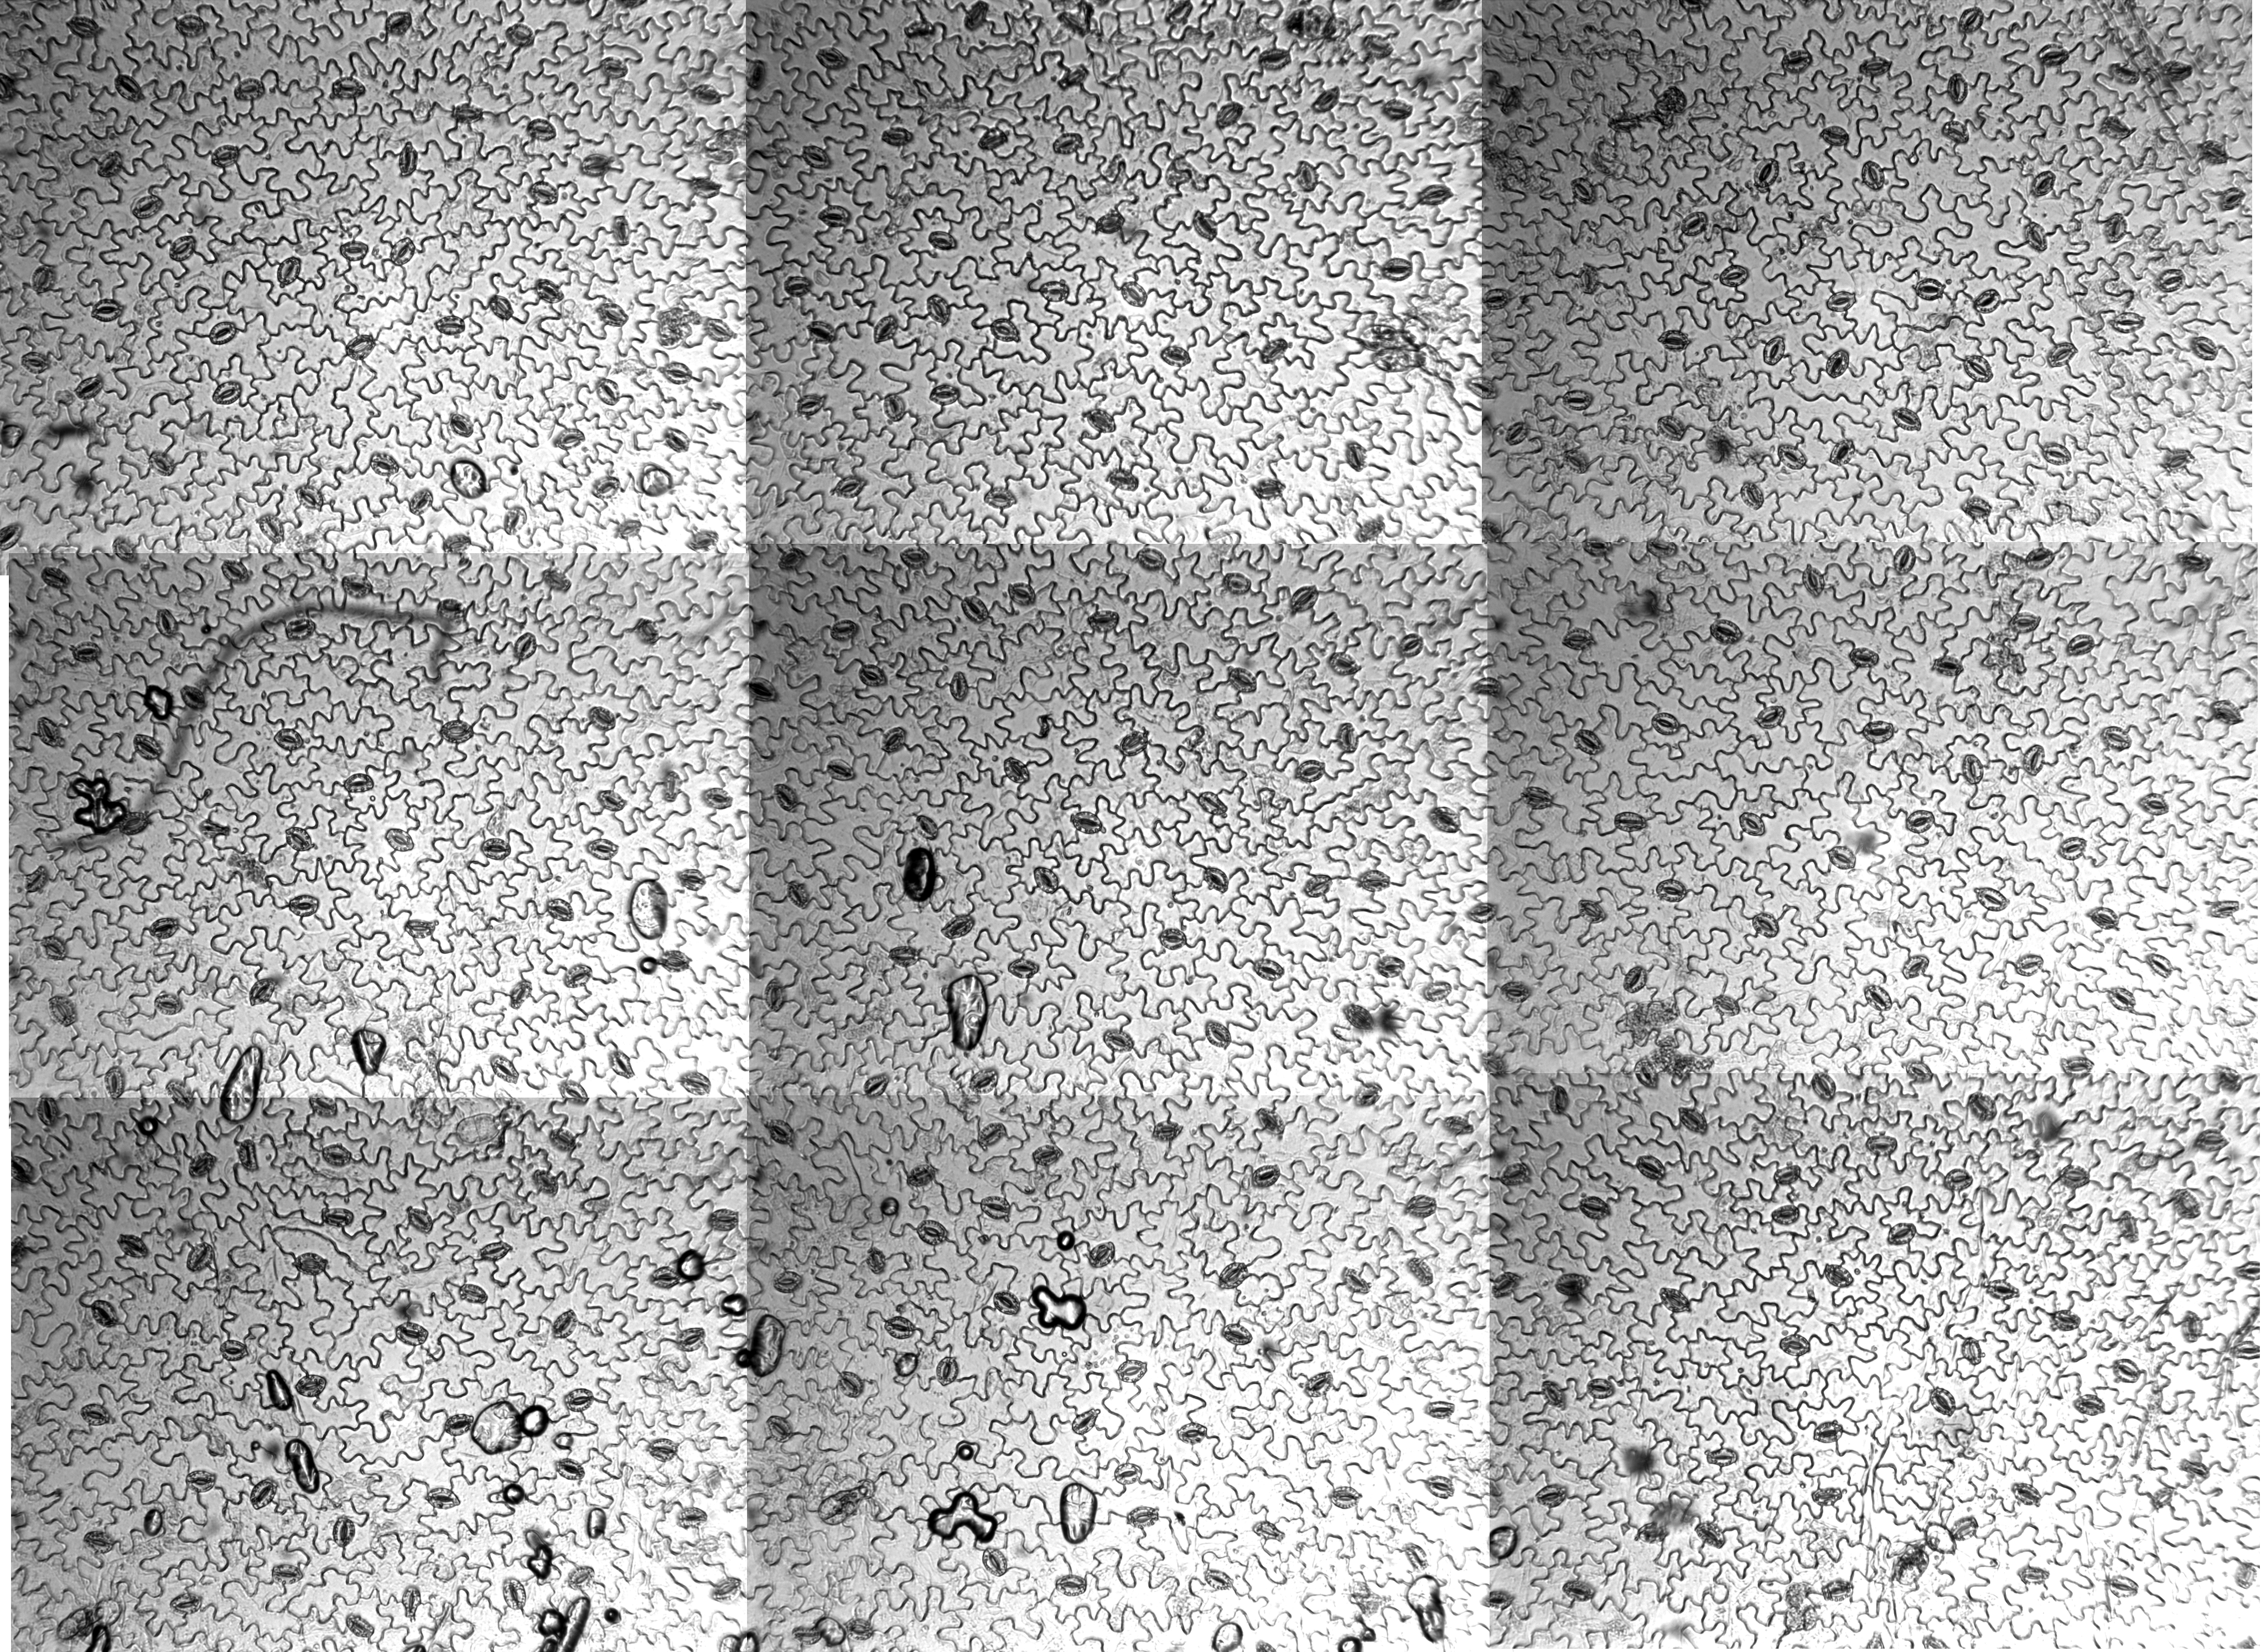
\includegraphics[width=\textwidth]{ch5_figs/stoma}
  \caption{Original Stomatal Array Image}
  \end{subfigure}
  
  \begin{subfigure}[t]{0.6\textwidth}
  \centering
  \includegraphics[width=\textwidth]{ch5_figs/stoma-colored}
  \caption{Stomatal Array with Stomata Marked}
  \end{subfigure}
  
  \begin{subfigure}[t]{0.6\textwidth}
  \centering
  \includegraphics[width=\textwidth]{ch5_figs/stoma_red_edited}
  \caption{Stomatal Delaunay Triangulation}
  \end{subfigure}
\caption[Grid Generation from Stomatal Array]{
  An illustration of the process we use to generate a grid from a stomatal array image. The final grid pictured is the Delaunay Triangulation of the generator points, which corresponds to the connectivity graph we utilize for the majority task CA.
  }
\label{fig:stoma_graph_gen}
\end{figure}

\subsubsection*{Results}
First we replicated \citeauthor{me07}'s baseline experiments to confirm the accuracy of our system, with our results corresponding exactly with theirs (Figure~\ref{fig:me07_baseline_rep}). The general profile of the Local Majority Task performance curve is symmetric, with a severe fall-off in task performance at around ON:OFF ratios of 15:85 and 85:15 and 0\% task performance between ratios of about 30:70 to 70:30. Since the majority classification tasks become increasingly difficult as the ON:OFF ratio approaches 50:50, this degradation in performance is to be expected for such a simple rule. For comparison, the task performance of a more complex rule table created through the use of a \textit{genetic algorithm} is also pictured in Figure~\ref{fig:me07_baseline}. The overall performance of this rule table is much better than the local majority rule, but also sees a drop in performance when classifying 50:50 initial ratios.

\begin{figure}[htp]
\centering
  \begin{subfigure}[t]{0.85\textwidth}
  \includegraphics[width=\textwidth]{ch5_figs/me07_fig2_LMBaseline}
  \caption{\citeauthor{me07}'s Baseline Local Majority Task Performance Graph}
  \label{fig:me07_baseline}
  \end{subfigure}

  \begin{subfigure}[t]{0.85\textwidth}
  \centering
  \includegraphics[width=\textwidth]{ch5_figs/lm_baseline_reg_tor}
  \caption{Replicated Baseline Local Majority Task Performance}
  \end{subfigure}
\caption[Replication of \citeauthor{me07}'s Baseline Local Majority Performance]{
  An illustration of baseline Local Majority task performance on square, periodic 15 by 15 grid. We achieve the same performance graph as \citeauthor{me07}, which is labeled LM in Figure~\ref{fig:me07_baseline}. The performance graph labeled Sip in Figure~\ref{fig:me07_baseline} is from a CA rule table created through the use of a genetic algorithm~\cite{me07}.
}
\label{fig:me07_baseline_rep}
\end{figure}

The task performance of our two irregular grids are pictured in Figure~\ref{fig:lm_ireg}. We see that both irregular grids have the same symmetric task performance profile as the baseline regular grids. This result suggests that irregular grids could be suitable for supporting complex behavior comparable to regular grids. It is also important to note that both irregular grids lack periodic boundary conditions unlike the baseline regular case. The absence of periodicity decreases neighborhood connectivity and will hurt a CA's ability to transfer information across the grid space, making the task performance of the irregular grids even more remarkable. For comparison, local majority task performance for regular grid is reduced significantly when periodic boundary conditions are removed, shown in Figure~\ref{fig:lm_reg_nonper}. Thus, it appears that in the context of the majority task, spatial irregularity will not hinder the performance or behavior of a CA system. The fact that local majority task performance is essentially equivalent across both square and spatially irregular grids establishes a rough form of equivalence between the two grid types within the domain of the CA majority task.

\begin{figure}[htp]
\centering
  \begin{subfigure}[t]{0.6\textwidth}
  \includegraphics[width=\textwidth]{ch5_figs/LM_baseline_vor}
  \caption{Local Majority Task Performance on a Voronoi Grid}
  \end{subfigure}
  ~
  \begin{subfigure}[t]{0.6\textwidth}
  \centering
  \includegraphics[width=\textwidth]{ch5_figs/lm_baseline_stoma}
  \caption{Local Majority Task Performance on a Stoma Grid}
  \end{subfigure}
\caption[Local Majority Task Performance on Irregular Grids]{
  Task Performance graphs for both our generated irregular grid and the stoma irregular grid. Both have almost identical performance profiles to the baseline Local Majority task performance graph for regular grids.
}
\label{fig:lm_ireg}
\end{figure}

\begin{figure}[htp]
\centering
\includegraphics[width=0.6\textwidth]{ch5_figs/lm_baseline_reg_nontor}
\caption[Local Majority Task Performance on a Non-Periodic Regular Grid]{
  The task performance graph for a 15 by 15 regular grid with non-periodic boundary conditions. Notice the degradation in task performance in comparison to the performance graphs in Figure~\ref{fig:me07_baseline_rep}.
}
\label{fig:lm_reg_nonper}
\end{figure}

\subsection{Majority Task Performance with State Noise}

\citeauthor{me07} discovered in their investigations that introducing small amounts of state noise improves the performance of majority task CA, likely due to the fact that the random state change will stimulate movement across the grid~\cite{me07}. We will investigate the impact of state noise in more detail and in the context of irregular grids. 

\subsubsection*{Experimental Setup}

Data for task performance graphs is collected with the same setup and number of trials as in the previous section. State noise is introduced by changing each cell's correct output state with probability $\eta$ before the next timestep. State noise is not applied if the CA has reached a uniform configuration of either all ON or all OFF states. Since \citeauthor{me07} reported that state noise probabilities of $\eta \ge 0.1$ caused massive degradation of majority task performance, we consider a range of state noise from $\eta=0.01$ to $\eta=0.15$.

Since initial ON:OFF ratios near 50:50 are the most difficult starting configurations to classify, we also perform experiments that measure the impact of state noise on ``hard'' initial configurations. For each state noise percentage, we generate 1,000 random initial configurations with ON:OFF ratios chosen from a Gaussian distribution $\mathcal{N}(0.5, 0.06)$.

\subsubsection*{Results}

Task performance graphs for regular grids with state noise $\eta=0.05$ and $\eta=0.15$ are shown in Figure~\ref{fig:lm_reg_noise}. We see that with an introduction of a small amount of noise ($\eta=0.05$) task performance dramatically improves, with incorrect classifications only occurring between ON:OFF ratios of 40:60 and 60:40 and with roughly 35\% correct classifications of 50:50 starting ratios. Conversely, when too much noise is introduced to the system ($\eta=0.15$), task performance across all starting ratios degrade below baseline levels. The task performance graphs for the irregular stoma grid with $\eta=0.05, 0.15$ also exhibit the same trend (Figure~\ref{fig:lm_stoma_noise}). However, for the stoma grid with $\eta=0.05$ only about 10\% of the 50:50 starting ratios are correctly classified, which is poorer performance on 50:50 configurations compared to the regular grid. Overall however, the regular and irregular grids exhibit the same sort of behavior when varying levels of state noise are applied. With the addition of small amounts of state noise, the basic Local Majority rule table performs similarly to more complex rule tables; the performance graph for both regular and irregular grids at $\eta=0.05$ closely resembles the performance graph of the Sip rule pictured in Figure~\ref{fig:me07_baseline}, one of the best performing rule tables evaluated by \citeauthor{me07}~\cite{me07}.

\begin{figure}[htp]
\centering
  \begin{subfigure}[t]{0.85\textwidth}
  \includegraphics[width=\textwidth]{ch5_figs/baseline_noise_5}
  \caption{Local Majority Task Performance on a Regular Grid with 5\% Noise}
  \end{subfigure}
  ~
  \begin{subfigure}[t]{0.85\textwidth}
  \centering
  \includegraphics[width=\textwidth]{ch5_figs/baseline_noise_15}
  \caption{Local Majority Task Performance on a Regular Grid with 15\% Noise}
  \end{subfigure}
\caption[Local Majority Task Performance for Regular Grids with Noise]{
  Majority Task Performance graphs for regular grids with state noise $\eta = 0.05, 0.15$. Note the relative increase and decrease in task performance for low and high amounts of noise, respectively.
}
\label{fig:lm_reg_noise}
\end{figure}

\begin{figure}[htp]
\centering
  \begin{subfigure}[t]{0.85\textwidth}
  \includegraphics[width=\textwidth]{ch5_figs/stoma_noise_5}
  \caption{Local Majority Task Performance on the Stoma Grid with 5\% Noise}
  \end{subfigure}
  ~
  \begin{subfigure}[t]{0.85\textwidth}
  \centering
  \includegraphics[width=\textwidth]{ch5_figs/stoma_noise_15}
  \caption{Local Majority Task Performance on the Stoma Grid with 15\% Noise}
  \end{subfigure}
\caption[Local Majority Task Performance for the Stoma Grid with Noise]{
    Majority Task Performance graphs for the irregular stomata grid with state noise $\eta = 0.05, 0.15$. Note that though the shape of the two graphs resemble those in Figure~\ref{fig:lm_reg_noise}, the irregular $\eta=0.05$ graph has a sharper drop-off in 50:50 initial ratio task performance.
}
\label{fig:lm_stoma_noise}
\end{figure}

The results for local majority task performance on ``hard'' configurations on both regular and stoma grids are shown in Figure~\ref{fig:lm_ff}. We see that task performance significantly increases when state noise $\eta \ge 0.02$ and then quickly degrades when state noise $\eta \ge 0.12$ for both grids. In the regular case, task performance stays relatively steady just above 70\% when $0.02 \le \eta \le 0.12$ while in the irregular stomatal case task performance gradually rises to about 60\% correct classification in that same state noise range. These results confirm that small amounts of state noise is beneficial for majority task performance, regardless of the spatial dynamics of the grid. These results also confirm the viability of irregular Voronoi grids in supporting majority task behavior, with task performance on the stomatal grid closely resembling the results on regular grids throughout all these experiments.

\begin{figure}
\centering
  \begin{subfigure}[t]{0.85\textwidth}
  \includegraphics[width=\textwidth]{ch5_figs/ff_reg}
  \caption{Regular Grid Task Performance on Hard Configurations}
  \end{subfigure}
  ~
  \begin{subfigure}[t]{0.85\textwidth}
  \centering
  \includegraphics[width=\textwidth]{ch5_figs/ff_stoma}
  \caption{Stoma Grid Task Performance on Hard Configurations}
  \end{subfigure}
\caption[Local Majority Task Performance on ``Hard'' Configurations]{
  Local Majority task performance graphs on ``hard'' configurations for both regular grids and stoma grids. For both grids, task performance improves significantly between $\eta=0.02$ and $\eta=0.12$ before falling at $\eta \ge 0.12$. 
}
\label{fig:lm_ff}
\end{figure}

\subsection{Summary}
We have evaluated local majority task performance on both regular grids and irregular Voronoi grids. The profiles of the performance graphs show remarkable similarities between the regular and irregular grids in majority task performance. These similarities continue when we examine the impact of state noise, though the irregular grids perform slightly worse than the regular grids when noise is introduced. Still, we see that small amounts of state noise \textit{improve} task performance in both the regular and irregular grid cases, with their overall classification percentages rivaling those of more complex, human-engineered majority task rule tables.

Thus, we see more evidence that randomness can facilitate the function of decentralized dynamic systems, and it seems plausible that biological systems utilizing local communication can overcome spatial irregularity and perform comparably to ``perfect'' CA systems even in noisy environments. Again, we see some evidence that spatially irregular grids can be functionally equivalent to their regular counterparts within a specific CA task domain.

%\processdelayedfloats

\section{Lambda Degradation Experiments}
\label{sec:lambda_degen}
The $\lambda$ parameter as established by \citeauthor{la90} is an effective way to parameterize and traverse the CA rule space. And though $\lambda$ may be too ``coarse'' of a parameter to pinpoint precisely where the \textit{critical transition point} is for particular class of CAs (see Chapter~\ref{subsec:edge_chaos}), it is sufficient for detecting whether or not transition events can occur for a given CA. Thus, we apply similar $\lambda$ analysis techniques used by \citeauthor{wo90}~\cite{la90,wo90} to irregular and degraded grids.

\subsection{The Langton-Wootters $\lambda$ Profile}
Our experiments build off work by \citeauthor{wo90} that specifically examine $K=8, N=5$ CAs. As discussed in Chapter~\ref{subsec:metrics}, \textit{Shannon entropy} is often used to measure the complexity of CA systems. Entropy is plotted against $\lambda$ in \citeauthor{wo90}'s experiments to produce what we call the \textit{Langton-Wootters Profile} (LW Profile), pictured in various forms from different table generation methods in Figure~\ref{fig:lw_profile}.

\subsubsection*{Generating the Langton-Wootters Profile}

The \textit{table walk-through} method for generating transition tables begins with a $\Delta$ transition function that has $\lambda = 0$. Recalling the definition of $\lambda$ (Appendix~\ref{appA:lambda}), $\lambda=0$ indicates that every rule in $\Delta$ maps to the quiescent state $s_q$. The $\Delta$ table is then \textit{incremented} to a higher $\lambda$ value by randomly replacing some of the transitions to $s_q$ with transitions to the other possible states, uniformly chosen~\cite{la90}. This table generation method has the effect of modifying the ``same'' table, allowing us to track CA behavior for individual runs of CA simulation. The LW Profile generated from the table walk-through method is shown in Figure~\ref{fig:lw_profile_walk}.

The \textit{random table} method for generating transition tables utilizes $\lambda$ as a sampling probability. A $\Delta$ table entry is mapped to the quiescent state with probability $1 - \lambda$, while a non-quiescent state is chosen uniformly from the other possible states with probability $\lambda$~\cite{la90}. The LW Profile generated from the random table method is pictured in Figure~\ref{fig:lw_profile_rand}. Also note that all $\Delta$ transition tables possess \textit{planar isotropy} and \textit{strong quiescence} as detailed in Chapter~\ref{subsec:ch3_lamb}.

Entropy is calculated using the equations shown in Appendix~\ref{appA:entrop}. However, entropy calculations are made only for the asymptotic behavior of a given CA simulation: each CA simulation is run for 1,000 time steps, with entropy only measured after time step 500. So if a particular CA run has a lifetime of less than 500, its entropy value will be 0. This manner of calculating asymptotic entropy leads to numerous entropy measurements of 0, as pictured in both versions of the LW Profile. Also note that for $K=8, N=5$ CA, the maximum entropy is 3 with this maximum value occurring with a $\lambda$ value of 0.875 (Appendix~\ref{appB:max_H}). Thus, all experiments with $K=8, N=5$ CA consider a range of $\lambda$ values from $\lambda = 0.0$ to $\lambda = 0.88$. 

\begin{figure}[htp]
\centering
  \begin{subfigure}[t]{0.65\textwidth}
  \includegraphics[width=\textwidth]{ch6_figs/la90_fig8_lambda_runs}
  \caption{Walk-Through Langton-Wootters Profile}
  \label{fig:lw_profile_walk}
  \end{subfigure}
  ~
  \begin{subfigure}[t]{0.65\textwidth}
  \centering
  \includegraphics[width=\textwidth]{ch6_figs/wo90_fig3_entropy_lambda}
  \caption{Random Table and Theoretical Langton-Wootters Profile}
  \label{fig:lw_profile_rand}
  \end{subfigure}
\caption[The Langton-Wootters Profile]{
  Different forms of the LW Profile. Figure~\ref{fig:lw_profile_walk} shows 50 individual runs of the table-walk-through method of varying $\lambda$. Figure~\ref{fig:lw_profile_rand} shows both a scatter plot of data points collected through the random-table method of varying $\lambda$ and the theoretical Langton-Wootters Profile as predicted by mean field theory (Appendix~\ref{appA:MFT}). Note how both plots produce the same envelope of data points. Plots adapted from both \citeauthor{wo90}, and \citeauthor{la90}~\cite{la90,wo90}.
}
\label{fig:lw_profile}
\end{figure}

\subsubsection*{Analysis of the Langton-Wootters Profile}

Both renditions of the LW Profile indicate a bimodal distribution of entropy values, with most data points either collected around $H=0$ or $H > 0.85$. There is a region where relatively few data points are observed over $0 \le \lambda \le 0.6$ and $0 < H \le 0.85$. This \textit{transition gap} and bimodal distribution are indicators of a critical transition, illustrating the boundary between non-complex CA with low $H$ values and complex CA with much higher $H$ values. This phenomenon is easy to see in Figure~\ref{fig:lw_profile_walk}, with individual transition table runs showing a sharp increase in entropy from below the gap to above the gap at a certain $\lambda$ value. This gap and sudden jump in $H$ are indications that critical transitions can occur in this particular class of CAs on regular grids. Thus, we will utilize these features of the LW Profile to evaluate irregular grids on their ability to support complex behavior. 
Also observe that entropy values converge rapidly when $\lambda > 0.6$, an indication of the shift of rule tables from complex (Class IV CA) to chaotic (Class III CA). The most interesting action occurs when the variance of entropy values is high, again corresponding to the critical transition gap and jump in entropy from around $H=0.0$ to $H > 0.85$. \citeauthor{la90} discusses the ``ceiling'' of this transition region, noting that $H \approx 0.84$ is the average entropy value of a commonly occurring low $\lambda$ chaotic rule~\cite{la90}, another indication that the gap in data points for $0 < H \le 0.85$ is indicative of a critical transition.

\subsection{$\lambda$ Profile of Irregular Grids}

\subsubsection*{Experimental Setup}

We utilize the table walk-through method when varying $\lambda$ for our experiments, as both line and scatter plots can be generated from the resulting data. Though \citeauthor{wo90} run their CA simulations to 1,000 time steps, we saw no difference in the shape of the LW Profiles between trials with a maximum time step of 500 and trials with a maximum time step of 1,000 (Figure~\ref{fig:lw_reg_short_long}), so in the interest of efficiency we run our experiments with a maximum of 500 time steps with an asymptotic threshold of 250 time steps. 100 individual table walk-through runs for $K=8, N=5$ CA are made, incrementing $\lambda$ from $0.0$ to $0.88$. Since we are examining the $K=8, N=5$ CA class, we require the cells in our grid to have four neighbors. Thus, grids generated with the Voronoi Quadrilateral technique as discussed in Chapter~\ref{subsec:vquad} are appropriate irregular spaces for considering these CA. We apply the VQuad grid generation technique to a Voronoi diagram generated by a Poisson Disk distribution of generator points and to the Voronoi diagram produced by the stomatal array (Figure~\ref{fig:vquad_stoma_gen}). Additionally, we also examine Penrose grids utilizing the generalized von Neumann neighborhood stencil, which also produces neighborhoods of $N=5$. Both Kite/Dart and Thin/Thick Rhomb grids are considered, as shown in Figure~\ref{fig:penrose_circ}.

With irregular grids, inducing periodic boundary conditions is not obvious, so boundary cell neighborhoods are ``completed'' by inserting quiescent states. Note that this decision could potentially skew the resultant entropy measurements lower, but we have seen some functional equivalence between periodic and non-periodic grids previously with our experiments in Chapter~\ref{sec:local_maj}. Neighborhood cells are ordered clockwise from the origin; since the $\lambda$ rule tables produced are isotropic, only the relative ordering of neighborhood cells matter. Cell state frequencies are measured at every time step, so entropy values are computed as an average over the data points collected after the asymptotic threshold.

\begin{figure}[htp]
\centering
  \begin{subfigure}[t]{0.8\textwidth}
  \includegraphics[width=\textwidth]{ch6_figs/v_stoma_edited}
  \caption{Voronoi Diagram of Stomatal Array}
  \end{subfigure}
  ~
  \begin{subfigure}[t]{0.8\textwidth}
  \centering
  \includegraphics[width=\textwidth]{ch6_figs/q_stoma}
  \caption{VQuad Diagram of Stomatal Array}
  \end{subfigure}
\caption[VQuad Generation from Stomatal Array]{
An illustration of the Voronoi representation of the stomatal array from Figure~\ref{fig:stoma_graph_gen} and the resultant Voronoi Quad grid. 
}
\label{fig:vquad_stoma_gen}
\end{figure}

\begin{figure}[htp]
\centering
  \begin{subfigure}[t]{0.65\textwidth}
  \includegraphics[width=\textwidth]{ch6_figs/reg_entropy_500_scatter}
  \caption{Short Simulation ($t_{max} = 500$) Langton-Wootters Profile}
  \label{fig:lw_profile_short}
  \end{subfigure}
  ~
  \begin{subfigure}[t]{0.65\textwidth}
  \centering
  \includegraphics[width=\textwidth]{ch6_figs/reg_entropy_1000_scatter}
  \caption{Long Simulation ($t_{max} = 1000$) Langton-Wootters Profile}
  \label{fig:lw_profile_long}
  \end{subfigure}
\caption[Langton-Wootters Profile for Short and Long Simulations]{
  LW Profiles for both short and long simulations. The overall shape and distribution of data points throughout the graph are largely identical. Thus, it appears that equivalent asymptotic behavior can be achieved within different time scales. Note that in our scatter plots, darker dots indicate higher frequency of values. So, we can see both the tight convergence of entropy at high $\lambda$ values and the high frequency of runs that do not reach the asymptotic threshold, resulting in an entropy value of 0.
}
\label{fig:lw_reg_short_long}
\end{figure}

\subsection*{Results}

The LW Profiles for our Poisson Disk and Stomatal Voronoi Quad grids are pictured in Figure~\ref{fig:vor_lw_profile} and Figure~\ref{fig:stoma_lw_profile} respectively. In both cases, despite the irregularity in the cell orientation and the non-periodic boundary conditions, we see a remarkably similar shape in the LW Profile for the Voronoi Quad grids. Examination of Figures \ref{fig:vor_lw_run} and \ref{fig:stoma_lw_run} show all of the individual CA runs experiencing a significant jump in entropy values at some point, evidence of a transition event. The corresponding scatter plots (Figures \ref{fig:vor_lw_scatter} and \ref{fig:stoma_lw_scatter}) of these graphs show that the transition gap in $0 < H \le 0.85$ is also sparsely populated. There appear to be slightly more data points found in the gap for the stoma grid scatter plot compared to the Poisson Disk grid plot; we speculate that the size of the grid may have an influence on a CA's ability to compute, and the Poisson Disk grid is significantly larger than the stomatal grid. 

LW Profiles for the Penrose tilings are pictured in Figure~\ref{fig:penrose_lw_profile}. Though the overall shape of the curves are still in line with the baseline profile, we see some small deviations in the LW Profile for Rhomb tilings, shown in Figure~\ref{fig:crh_lw_profile}. First, we see that the transition gap contains a fair amount of data points, spanning a much larger range of $\lambda$ than any of the other grids we have examined with points in the gap found at $\lambda < 0.2$. There is also more variance in the data points above the transition gap, producing a slightly looser convergence of entropy as $\lambda$ increases. These discrepancies are surprising given our Penrose Life experiments in Chapter~\ref{ch:penrose} showing that the Rhomb tilings supported longer lived structures, which suggests that the grids would be better suited for supporting complex behavior. Thus, there is a need for a way to quantify how these graphs may differ from one another, as visual inspection is not an adequate measure of such differences. Overall however, we see entropy profile behavior equivalent to those seen in the baseline experiments as we vary $\lambda$ across all of these irregular grids, suggesting a functional equivalence between irregular, non-periodic quadrilateral grids and their regular, periodic square counterparts. With the preservation of both the overall shape and a well-defined transition gap of the LW Profiles we have examined, it appears that complex behavior can be supported in all of these irregular quadrilateral grids.

\begin{figure}[htp]
\centering
\begin{subfigure}[t]{0.65\textwidth}
  \includegraphics[width=\textwidth]{ch6_figs/vor_entropy}
  \caption{VQuad Langton-Wootters Profile (Individual Runs)}
  \label{fig:vor_lw_run}
\end{subfigure}
~
\begin{subfigure}[t]{0.65\textwidth}
  \centering
  \includegraphics[width=\textwidth]{ch6_figs/vor_entropy_scatter}
  \caption{VQuad Langton-Wootters Profile (Scatter Plot)}
  \label{fig:vor_lw_scatter}
\end{subfigure}
\caption[Voronoi Quad Langton-Wootters Profile]{
  The LW Profile for a Voronoi Quad grid generated with a Poisson Disk distribution of 4,032 generator points resulting in a VQuad grid with 11,480 cells. Note how closely the scatter plot for the Voronoi Quad grid resembles the shape of the baseline LW Profile in Figure~\ref{fig:lw_profile}. There are very little points observed within the transition gap, and ceiling of the gap is sharply demarcated. It appears that despite the non-periodic boundary conditions and the irregular spatial distribution of grids, this Voronoi Quad grid is capable of supporting complex CA behavior.
}
\label{fig:vor_lw_profile}
\end{figure}

\begin{figure}[htp]
\centering
\begin{subfigure}[t]{0.65\textwidth}
  \includegraphics[width=\textwidth]{ch6_figs/stoma_entropy}
  \caption{Stoma Langton-Wootters Profile (Individual Runs)}
  \label{fig:stoma_lw_run}
\end{subfigure}
~
\begin{subfigure}[t]{0.65\textwidth}
  \centering
  \includegraphics[width=\textwidth]{ch6_figs/stoma_entropy_scatter}
  \caption{Stoma Langton-Wootters Profile (Scatter Plot)}
  \label{fig:stoma_lw_scatter}
  \end{subfigure}
\caption[Stoma Langton-Wootters Profile]{
  The LW Profile for the Voronoi Quad grid generated from the plant stomatal array (Figure~\ref{fig:vquad_stoma_gen}) resulting in 984 total cells. Like the Poisson Disk VQuad grid, we see a strong resemblance between the overall shape of the graph with the baseline LW Profile with Figure~\ref{fig:stoma_lw_run} showing the large transition jumps in entropy seen in Figure~\ref{fig:lw_profile}. We do see more ``noise'' within the transition gap region compared to Figure~\ref{fig:vor_lw_scatter}. The size of the grid may be a factor in supporting complex behavior, as the stomatal grid is significantly smaller than the Poisson Disk grid. Still, the equivalence in shape of this plot to the baseline suggests that this stomatal grid can also support complex, class IV CAs.
}
\label{fig:stoma_lw_profile}
\end{figure}

\begin{figure}[htp]
\centering
\begin{subfigure}[t]{0.65\textwidth}
  \includegraphics[width=\textwidth]{ch6_figs/ckd_entropy_scatter}
  \caption{Kite/Dart Langton-Wootters Profile}
  \label{fig:ckd_lw_profile}
\end{subfigure}
~
\begin{subfigure}[t]{0.65\textwidth}
  \centering
  \includegraphics[width=\textwidth]{ch6_figs/crh_entropy_scatter}
  \caption{Thin/Thick Rhombus Langton-Wootters Profile}
  \label{fig:crh_lw_profile}
  \end{subfigure}
\caption[Penrose Langton-Wootters Profile]{
  The LW Profile for both types of Penrose grids. Though both plots maintain the same overall shape as the baseline LW Profile, there appears to be significantly more noise throughout the entire graph for the Rhomb grid, with more points within the transition gap and looser convergence to the overall profile shape at entropy values above the transition gap. This is surprising given that our Penrose Life experiments showed the Rhomb tilings supporting longer living Life structures than the Kites/Dart tiling, suggesting that perhaps the Rhomb tilings would be better suited for supporting complex CA behavior in general.
}
\label{fig:penrose_lw_profile}
\end{figure}

\subsection{$\lambda$ Profile of Degenerated Grids}

Now that some equivalence in CA behavior has been established for our irregular grids, we want to examine how these grids respond to degradation. We expose CA systems to other forms of spatial irregularity through introducing ``internal'' boundaries by removing cells and through isolating local regions by reducing neighborhood connectivity. Our goal is to examine how robust cellular automata can be when facing spatial deterioration, another form of environmental noise (see Chapter~\ref{sec:Robust}) natural systems have to combat.

\subsection{Generator Point Degeneration}
\label{subsec:ch6_gen_pt_degen}
\subsubsection*{Experimental Setup}
We introduce internal boundary conditions by removing cells through the generator point removal technique outlined in Chapter~\ref{subsec:gen_pt_rem}. We apply degeneration percentages of $0.05,0.1, 0.15, 0.20$ to our stomatal Voronoi Quad grid, seen in Figure~\ref{fig:stoma_gen_pt_degen}. We then perform the same $\lambda$ experiments from the previous section, running simulations of $\lambda=0.01$ to $\lambda=0.87$ with $t_{max} = 500$ and the asymptotic threshold at $t=250$ for 100 total trials. 

\begin{figure}[htp]
\centering
\begin{subfigure}[t]{0.45\textwidth}
  \includegraphics[width=\textwidth]{ch6_figs/degen_stoma_5_grid}
  \caption{5\% Generator Point Degeneration}
\end{subfigure}
~
\begin{subfigure}[t]{0.45\textwidth}
  \centering
  \includegraphics[width=\textwidth]{ch6_figs/degen_stoma_10_grid}
  \caption{10\% Generator Point Degeneration}
  \end{subfigure}

\begin{subfigure}[t]{0.45\textwidth}
  \centering
  \includegraphics[width=\textwidth]{ch6_figs/degen_stoma_15_grid}
  \caption{15\% Generator Point Degeneration}
  \end{subfigure}
~
\begin{subfigure}[t]{0.45\textwidth}
  \centering
  \includegraphics[width=\textwidth]{ch6_figs/degen_stoma_20_grid}
  \caption{20\% Generator Point Degeneration}
  \label{fig:stoma_gen_pt_20}
  \end{subfigure}

\caption[Stomatal Generator Point Degeneration]{
  Representative degenerated Stomatal Grids through generator point removal. Notice how the generator point removal method causes relatively large areas of cells to be erased; there are no single cell removals as a result of this degeneration technique. With randomized generator point deletion, it is difficult for regions of the grid to be completely isolated. Even with a significant number of generator points removed, the remaining cells shown in Figure~\ref{fig:stoma_gen_pt_20} still form a completely connected grid.
}
\label{fig:stoma_gen_pt_degen}
\end{figure}

\subsubsection*{Results}

The resulting LW Profiles are pictured in Figure~\ref{fig:lw_gen_pt_degen}. We see that at 5\% degeneration (Figure~\ref{fig:lw_degen_pt_5}), the overall profile structure is largely unchanged from the non-degraded LW Profile for the stoma grid (Figure~\ref{fig:stoma_lw_scatter}) with only a slightly looser convergence at higher entropy values being observed. We see similar results at 10\% and 15\% degeneration as well, with looser convergence and an increase in data points found within the transition gap. However, for all three of these graphs we still see a clear demarcation of the transition gap itself as well as the preservation of the overall profile shape. It appears that transition events can occur even with relatively large amounts of spatial deterioration introduced, showing that CA systems can be robust and degrade gracefully. However, there is a breaking point, as we see in Figure~\ref{fig:lw_degen_pt_20} at 20\% degeneration: the transition gap completely collapses, with many data points observed within the $0 < H \le 0.85$ range. We also see very loose convergence of $H$, even at higher $\lambda$. The grid in this case has suffered too much damage and is now incapable of supporting complex behavior. From visual inspection, we speculate that the 20\% degeneration made information transfer across the space too difficult for complex behavior to be facilitated. Still, it is remarkable that complex CA systems could still functionally operate with as much as 15\% deterioration applied to the grid.


\begin{figure}[htp]
\centering
\begin{subfigure}[t]{0.4\textwidth}
  \includegraphics[width=\textwidth]{ch6_figs/degen_stoma_5}
  \caption{LW Profile, 5\% Degeneration}
  \label{fig:lw_degen_pt_5}
\end{subfigure}
~
\begin{subfigure}[t]{0.4\textwidth}
  \centering
  \includegraphics[width=\textwidth]{ch6_figs/degen_stoma_10}
  \caption{LW Profile, 10\% Degeneration}
  \label{fig:lw_degen_pt_10}
  \end{subfigure}

\begin{subfigure}[t]{0.4\textwidth}
  \centering
  \includegraphics[width=\textwidth]{ch6_figs/degen_stoma_15}
  \caption{LW Profile, 15\% Degeneration}
  \label{fig:lw_degen_pt_15}
  \end{subfigure}
~
\begin{subfigure}[t]{0.4\textwidth}
  \centering
  \includegraphics[width=\textwidth]{ch6_figs/degen_stoma_20}
  \caption{LW Profile, 20\% Degeneration}
  \label{fig:lw_degen_pt_20}
  \end{subfigure}

\caption[Langton-Wootters Profile for Generator Point Degeneration]{
  LW Profiles for generator point degeneration. Notice that the shape of the profile as well as the transition gap is maintained at 5\% degeneration. The preservation of the overall structure of the profile continues at both 10\% and 15\% degeneration, with only more noise being observed within the transition gap. At 20\% degeneration however, the ceiling of the transition gap collapses, losing both the well-defined boundaries of the gap as well as introducing significant noise within the region where $0 < H \le 0.85$.
}
\label{fig:lw_gen_pt_degen}
\end{figure}

\subsection{Crosshatching Degeneration}

In the previous section, we degraded a CA grid by randomly deleting cells from it. In order to more tightly control how spatial degeneration occurred throughout the grid, we utilize the \textit{crosshatching degeneration} method described in Chapter~\ref{subsec:ch_degen}. With this technique, we can vary how isolated local regions are within the grid without having to explicitly remove cells. This allows us to investigate the role of both overall grid size and connectivity in supporting complex CA behavior.

\subsubsection*{Experimental Setup}
Crosshatching degeneration is applied to our stomatal VQuad grid with crosshatch widths of $w=10,15,20,25,30$. The edge removal probability $p$ ranges from $p=0.05$ to $p=1.0$, in increments of $0.05$. We degenerate the grid for each $\lambda$ trial, producing new crosshatchings for every run, with examples in Figures \ref{fig:ch_w10_grid}, \ref{fig:ch_w20_grid}, and \ref{fig:ch_w30_grid}. Otherwise, $\lambda$ experiments are run in an identical manner as the previous two sections, with 100 trials varying $\lambda$ from $\lambda=0.01$ to $\lambda=0.88$.

\begin{figure}[htp]
\centering
\begin{subfigure}[t]{0.45\textwidth}
  \includegraphics[width=\textwidth]{ch6_figs/cross_hatch_p25_w10}
  \caption{Crosshatch Degeneration, $w=10$, $p=0.25$}

\end{subfigure}
~
\begin{subfigure}[t]{0.45\textwidth}
  \centering
  \includegraphics[width=\textwidth]{ch6_figs/cross_hatch_p50_w10}
  \caption{Crosshatch Degeneration, $w=10$, $p=0.50$}

  \end{subfigure}

\begin{subfigure}[t]{0.45\textwidth}
  \centering
  \includegraphics[width=\textwidth]{ch6_figs/cross_hatch_p75_w10}
  \caption{Crosshatch Degeneration, $w=10$, $p=0.75$}

  \end{subfigure}
~
\begin{subfigure}[t]{0.45\textwidth}
  \centering
  \includegraphics[width=\textwidth]{ch6_figs/cross_hatch_p100_w10}
  \caption{Crosshatch Degeneration, $w=10$, $p=1.0$}

  \end{subfigure}

\caption[Crosshatch Degeneration, $w=10$]{
  Representative grids for crosshatching degeneration $w=10$ applied to the stomatal VQuad grid. Notice how at $p=1.0$, the crosshatchings are placed so close together that subregion partitions are not well-defined.
}
\label{fig:ch_w10_grid}
\end{figure}

\begin{figure}[htp]
\centering
\begin{subfigure}[t]{0.45\textwidth}
  \includegraphics[width=\textwidth]{ch6_figs/cross_hatch_p25_w20}
  \caption{Crosshatch Degeneration, $w=20$, $p=0.25$}

\end{subfigure}
~
\begin{subfigure}[t]{0.45\textwidth}
  \centering
  \includegraphics[width=\textwidth]{ch6_figs/cross_hatch_p50_w20}
  \caption{Crosshatch Degeneration, $w=20$, $p=0.50$}

  \end{subfigure}

\begin{subfigure}[t]{0.45\textwidth}
  \centering
  \includegraphics[width=\textwidth]{ch6_figs/cross_hatch_p75_w20}
  \caption{Crosshatch Degeneration, $w=20$, $p=0.75$}

  \end{subfigure}
~
\begin{subfigure}[t]{0.45\textwidth}
  \centering
  \includegraphics[width=\textwidth]{ch6_figs/cross_hatch_p100_w20}
  \caption{Crosshatch Degeneration, $w=20$, $p=1.0$}

  \end{subfigure}

\caption[Crosshatch Degeneration, $w=20$]{
  Representative grids for crosshatching degeneration $w=20$ applied to the stomatal VQuad grid. As opposed to the $w=10$ case, when $p=1.0$ the crosshatchings partition the grid into clear subregion ``boxes.''
}
\label{fig:ch_w20_grid}
\end{figure}

\begin{figure}[htp]
\centering
\begin{subfigure}[t]{0.45\textwidth}
  \includegraphics[width=\textwidth]{ch6_figs/cross_hatch_p25_w30}
  \caption{Crosshatch Degeneration, $w=30$, $p=0.25$}

\end{subfigure}
~
\begin{subfigure}[t]{0.45\textwidth}
  \centering
  \includegraphics[width=\textwidth]{ch6_figs/cross_hatch_p50_w30}
  \caption{Crosshatch Degeneration, $w=30$, $p=0.50$}

  \end{subfigure}

\begin{subfigure}[t]{0.45\textwidth}
  \centering
  \includegraphics[width=\textwidth]{ch6_figs/cross_hatch_p75_w30}
  \caption{Crosshatch Degeneration, $w=30$, $p=0.75$}

  \end{subfigure}
~
\begin{subfigure}[t]{0.45\textwidth}
  \centering
  \includegraphics[width=\textwidth]{ch6_figs/cross_hatch_p100_w30}
  \caption{Crosshatch Degeneration, $w=30$, $p=1.0$}

  \end{subfigure}

\caption[Crosshatch Degeneration, $w=30$]{
  Representative grids for crosshatching degeneration $w=20$ applied to the stomatal VQuad grid. Again when $p=1.0$, the crosshatchings partition the grid into square subregions.
}
\label{fig:ch_w30_grid}
\end{figure}


\subsubsection*{Qualitative Analysis}

Representative entropy profiles are shown in Figures \ref{fig:lw_ch_10}, \ref{fig:lw_ch_20}, and \ref{fig:lw_ch_30} for \linebreak $w=10,20,30$, respectively. In the $w=10$ case, we see massive degeneration of the structure of the grid in the $p=0.75$ (Figure~\ref{fig:lw_w10_p75}) and $p=1.0$ (Figure~\ref{fig:lw_w10_p100}) graphs, with a loss of both the convergence of entropy values as well as the well-defined transition gap; if we look back to Figure~\ref{fig:ch_w10_grid}, we see that at $p=0.75$ and $p=1.0$ there is widespread edge removal across the entire grid with very little contiguous grid regions. This sort of damage is too much for a CA to overcome, and critical transitions are not observed on these grids. 

As the width of the crosshatching increases however, we see much more robust behavior. When $w=20$, we see preservation of the baseline LW Profile structure across all $p$ values, with only a slight weakening of convergence when $w=1.0$ (Figure~\ref{fig:lw_w20_p100}). Again the entropy profile structure is maintained when $w=30$, with tight convergence even when $w=1.0$. As the crosshatching width increases, there are fewer edges being removed from the grid, and larger contiguous subregions of the grid are preserved. Thus, we expect CA behavior to be more robust to grid degradation as the crosshatching width increases. Though we have evaluated these results through visual inspection of the LW Profiles, we will explore a more quantitative manner of assessing CA behavior on damaged grids.

\begin{figure}[htp]
\centering
\begin{subfigure}[t]{0.4\textwidth}
  \includegraphics[width=\textwidth]{ch6_figs/ch_w10_p25_entropy_scatter}
  \caption{Crosshatch Degen, $w=10$, $p=0.25$}

\end{subfigure}
~
\begin{subfigure}[t]{0.4\textwidth}
  \centering
  \includegraphics[width=\textwidth]{ch6_figs/ch_w10_p50_entropy_scatter}
  \caption{Crosshatch Degen, $w=10$, $p=0.50$}

  \end{subfigure}

\begin{subfigure}[t]{0.4\textwidth}
  \centering
  \includegraphics[width=\textwidth]{ch6_figs/ch_w10_p75_entropy_scatter}
  \caption{Crosshatch Degen, $w=10$, $p=0.75$}
  \label{fig:lw_w10_p75}
  \end{subfigure}
~
\begin{subfigure}[t]{0.4\textwidth}
  \centering
  \includegraphics[width=\textwidth]{ch6_figs/ch_w10_p100_entropy_scatter}
  \caption{Crosshatch Degen, $w=10$, $p=1.0$}
  \label{fig:lw_w10_p100}
  \end{subfigure}

\caption[Crosshatch Langton-Wootters Profile, $w=10$]{
  LW Profile for $w=10$ Crosshatch Degeneration. Though the profiles resemble the baseline structure when $p=0.25$ and $p=0.5$, we see a large increase in the variance of entropy values, producing very loose convergence and the loss of a well-defined transition gap at $p=0.75$. For $p=1.0$ we see a complete collapse in the profile of the entropy graph; the grid is far too damaged to support complex CA behavior.
}
\label{fig:lw_ch_10}
\end{figure}

\begin{figure}[htp]
\centering
\begin{subfigure}[t]{0.4\textwidth}
  \includegraphics[width=\textwidth]{ch6_figs/ch_w20_p25_entropy_scatter}
  \caption{Crosshatch Degen, $w=20$, $p=0.25$}

\end{subfigure}
~
\begin{subfigure}[t]{0.4\textwidth}
  \centering
  \includegraphics[width=\textwidth]{ch6_figs/ch_w20_p50_entropy_scatter}
  \caption{Crosshatch Degen, $w=20$, $p=0.50$}

\end{subfigure}

\begin{subfigure}[t]{0.4\textwidth}
  \centering
  \includegraphics[width=\textwidth]{ch6_figs/ch_w20_p75_entropy_scatter}
  \caption{Crosshatch Degen, $w=20$, $p=0.75$}

  \end{subfigure}
~
\begin{subfigure}[t]{0.4\textwidth}
  \centering
  \includegraphics[width=\textwidth]{ch6_figs/ch_w20_p100_entropy_scatter}
  \caption{Crosshatch Degen, $w=20$, $p=1.0$}
  \label{fig:lw_w20_p100}
  \end{subfigure}

\caption[Crosshatch Langton-Wootters Profile, $w=20$]{
  LW Profile for $w=20$ Crosshatch Degeneration. We see a much better maintenance of the baseline structure through all $p$ compared to the $w=10$ case. We see a fair amount of noise in the transition gap throughout the four graphs, but the gap itself is well-defined in every case. Only at $p=1.0$ do we also see some ``sagging'' convergence of higher entropy values. Overall, CA systems appear able to perform adequately even with some subregions of the grid completely isolated from one another, provided that the subregions themselves are adequately large.
}
\label{fig:lw_ch_20}
\end{figure}

\begin{figure}[htp]
\centering
\begin{subfigure}[t]{0.4\textwidth}
  \includegraphics[width=\textwidth]{ch6_figs/ch_w30_p25_entropy_scatter}
  \caption{Crosshatch Degen, $w=30$, $p=0.25$}

\end{subfigure}
~
\begin{subfigure}[t]{0.4\textwidth}
  \centering
  \includegraphics[width=\textwidth]{ch6_figs/ch_w30_p50_entropy_scatter}
  \caption{Crosshatch Degen, $w=30$, $p=0.50$}

  \end{subfigure}

\begin{subfigure}[t]{0.4\textwidth}
  \centering
  \includegraphics[width=\textwidth]{ch6_figs/ch_w30_p75_entropy_scatter}
  \caption{Crosshatch Degen, $w=30$, $p=0.75$}

  \end{subfigure}
~
\begin{subfigure}[t]{0.4\textwidth}
  \centering
  \includegraphics[width=\textwidth]{ch6_figs/ch_w30_p100_entropy_scatter}
  \caption{Crosshatch Degen, $w=30$, $p=1.0$}
  \label{fig:lw_w30_p100}
  \end{subfigure}

\caption[Crosshatch Langton-Wootters Profile, $w=30$]{
  LW Profile for $w=30$ Crosshatch Degeneration. Again, overall structure of the entropy profile is maintained at all $p$, with the only deviations being data points observed in the transition gap. We see tight convergence of entropy values in all the graphs, even when $p=1.0$.  It appears that larger crosshatching widths impact the behavior of CA systems less; this is unsurprising as there are less edges removed from the grid and larger subregions being created as a result of the wider width.
}

\label{fig:lw_ch_30}
\end{figure}

\subsubsection*{Quantitative Analysis}
\label{subsec:ch6_mse}
We devised a measure that will quantify a given grid's ability to support computation or other complex behavior that utilizes mean field theory to provide a theoretical approximation of the LW Profile. Using the theoretical mean field theory approximation of entropy against $\lambda$ for $K=8, N=5$ cellular automata (Figure~\ref{fig:mft_lambda}), we calculate a given graph's \textit{mean squared error} (Equation~\ref{eq:mse}), measuring its deviation from the theoretical curve. Here, we are taking the expected value of the square distance between the estimated value $\hat{Y}$ and the actual observations $Y_i$. We use the MSE value of the standard periodic square grid as a baseline for comparison when we degrade the grid.

\begin{equation}
MSE = \frac{1}{n}\sum^n_{i=1}(\hat{Y}_i - Y_i)^2
\label{eq:mse}
\end{equation}

The MSE plot for all of our data is shown in Figure~\ref{fig:ch_mse}. Note that for $w=10$ and $w=15$ the increase of MSE is almost quadratic as $p$ increases. The extremely high MSE value for $w=10$, $p=1.0$ is to be expected if we look to its corresponding $\lambda$ profile (Figure~\ref{fig:lw_w10_p100}) and how far its shape deviates from the baseline profile. The MSE rate of increase decreases across all $p$ values as $w$ goes up however, and we see some confirmation of our qualitative analysis: the linear increase in MSE when $w \ge 20$ as opposed to a roughly quadratic increase corresponds to our previous observation that $\lambda$ profiles for $w \ge 20$ maintain the same overall baseline structure regardless of $p$. Overall, the use of MSE as a quantitative measure of critical behavior on CA grids seems informative, as structural features of a grid's $\lambda$ profile are appropriately represented in the MSE value. With these results, we hypothesize that CA systems have the ability to perform robustly even in the face of significant amounts of spatial irregularity. Of course, there is always a breaking point, but throughout our degradation experiments we have seen remarkable resilience of CA system performance on a myriad of irregular grids.


\begin{figure}[htp]
\centering
\includegraphics[width=\textwidth]{ch6_figs/ch_mse_10_30}
\caption[Mean Squared Error for Crosshatching Degeneration]{
  The Mean Square Error graph for our Crosshatching Degeneration experiments. We calculate average MSE over 100 trials for $p=0.10$ to $p=1.0$ with increments of $0.05$. The baseline value of $0.4234$ is the MSE for a 64 by 64 square periodic grid, the same parameters used for \citeauthor{wo90}'s initial $\lambda$ experiments. There is a rise in MSE as $p$ increases across all widths, but we see an almost quadratic increase in MSE for $w=10$; this is not surprising, given how many edges are removed from $w=10$ grids (Figure~\ref{fig:ch_w10_grid}) and how degraded their $\lambda$ profiles are at higher values of $p$ (Figure  \ref{fig:lw_ch_10}). However, the MSE rate of increase decreases as we raise $w$. From visual inspection of the $\lambda$ profiles it appeared that $w \ge 20$ grids can support transition events at all values of $p$ and indeed we see roughly linear increases of MSE for $w=20,30,40$ grids. Thus, it seems that MSE is a good approximation of a grid's ability to support CA transition events: in the context of the crosshatching degeneration, a linear increase in MSE as $p$ increases is indicative of such capability. 
}
\label{fig:ch_mse}
\end{figure}

\subsection{Summary}

Building upon the work done by \citeauthor{wo90}, we utilize $\lambda$ to parameterize the CA space and entropy to measure a CA system's complexity. We have seen the capacity for complex CA behavior across various irregular $N=5$ grids, despite the absence of periodic boundary conditions. We have also seen CA systems perform adequately even when exposed to imperfect, deteriorated grids. Through our quantitative analysis, we have also established MSE as a good approximation measure of a CA system's ability to support critical behavior on spatially irregular grids.

Now that we have seen how cellular automata respond to spatial irregularity, the next step would be to pinpoint specific characteristics that can impact a CA's ability to perform computation. Specifically, what are the conditions that render grids incapable of supporting complex behavior? In the instances we have examined, spatial irregularity has the potential to hinder information transfer across the grid space, which we observed in both our generator point and crosshatching experiments. The crosshatching experiments also revealed the importance of having contiguous subregions within the grid, as we saw robust critical behavior on grids with sufficiently wide crosshatches, even when regions of the grid were largely disconnected from one another. We speculate that spatial irregularity also impacts the ability of a CA system to store information; long lasting coherent structures, such as oscillators in GoL require space to ``take root'' within the grid in order to facilitate complex behavior. We have made a first step in investigating the impact of spatial irregularity on cellular automata function, and future work will look towards designing experiments and metrics that will consider these questions concerning the foundations of CA computation with more precision. 

%What are the conditions that render Grids incapable of supporting complex computation? Information transfer is important, but there also appear to be other factors (look to generator point degeneration and then the crosshatching degeneration).

%\processdelayedfloats

Throughout the previous chapters, we have considered how spatial irregularity impacts complex CA behavior. Our exploratory experiments have suggested that CA systems are relatively robust to nonuniform spatial environments and can even perform adequately on degraded or damaged grids. In some instances, we see that spatial irregularity even \textit{facilitates} complex behavior. However, all of these conclusions are qualified by the fact that we have only examined a few specific CA domains, utilizing metrics that are considered to capture broad, general characteristics of CA function rather than pinpointing specifics of \textit{critical} CA function. Thus, we will re-evaluate our results and consider some future directions expanding on the work we have done.

% \section{Evaluation and Critique of Our Results}

% Our experiments on Penrose Life, the Majority Task and $\lambda$ have all pointed to the idea that CA systems can operate on nonuniform grids. However, as we have noted in our discussions, there could be other properties that impact CA behavior that change alongside the spatial noise we introduce. The most prominent of such properties that we need to be aware of is neighborhood size. Previous work by \citeauthor{fl01} has suggested that the connectivity of a given cell is a major driving factor for variations on CA system behavior~\cite{fl01}, and the impact of irregular cells could simply be due to the introduction of variable neighborhood degree, not because of spatial non-uniformity itself. We see a similar sort of effect in the experiments we have run ourselves, as Penrose Life on Thin/Thick Rhomb grids had higher average lifetimes than on Kite/Dart grids (Chapter~\ref{ch4:lifetime}) but also had higher average neighborhood sizes (Chapter~\ref{sec:ch4_neighbors}) when using a generalized Moore neighborhood stencil. It is unclear what governs the Penrose Life average lifetimes in this situation, and when we consider Rhombs and Kites/Darts for $\lambda$ experiments with a von Neumann neighborhood (producing the same sized neighborhoods), we see that Kite/Dart grids perhaps support complex behavior better than Rhomb grids (Figure~\ref{fig:penrose_lw_profile}). Thus we need to carefully control the parameters of our experiments to ensure that connectivity and neighborhood size do not skew our results. Performing more experiments on specific classes of CAs, like our $\lambda$ investigations, where the neighborhood size is fixed is a good way to both parameterize the CA space and reduce any potential connectivity effects.

% Another characteristic of irregular grids we have to consider carefully is the grid boundary condition. Though traditional CA systems have the advantage of complete neighborhoods at every cell due to periodic square lattice boundaries, natural dynamic systems have to deal with the fact that some neighborhoods will be incomplete at the borders since they operate in a bounded space. We have seen that despite this limitation, CA systems on irregular grids can still perform comparably to their counterparts on regular, periodic grids.  We speculate that boundaries could act as regions of ``stability'' where neighborhood interactions are simpler and more consistent than within central regions of the grid: for example, we often saw long-living Penrose Life structures utilizing boundary cells to their advantage (Chapter~\ref{sec:ch4_single_run}). Then again, it is not clear how the boundary impacts a CA system's behavior in other domains, as majority task performance decreased on regular but non-periodic grids (Figure~\ref{fig:lm_reg_nonper}) in comparison to periodic grids, while irregular non-periodic grids perform comparably to the regular, periodic baseline case (Figure~\ref{fig:lm_ireg}). Internal boundary conditions must also be considered, as they are introduced when grids are spatially degraded, such as when cells are removed from the grid (Chapter~\ref{subsec:ch6_gen_pt_degen}). Ultimately, boundary conditions are unavoidable when considering spatial irregularities in natural dynamic systems and appear to play an important role in the type of CA behavior a space can support, so future experiments should isolate and attempt to distill the specific effects of a grid's boundary.

%\processdelayedfloats

\section{Conclusions}
\label{sec:Conclusion}
From the experiments we have conducted, we have tentatively shown that CA systems are robust to spatial irregularity. It appears that features of regular grids that initially seemed crucial for supporting CA behavior such as uniform neighborhood sizes and periodic boundaries are in fact not required for supporting complex behavior. Though we have relaxed many of the spatial assumptions made in traditional CA systems, both our majority task and $\lambda$ experiments have produced remarkably similar results to the regular grid case.

What do these findings tell us about equivalences between spatially different CA grids? Though our initial results are promising and suggest that there may at least be a rough functional equivalence between regular and irregular grids, more work has to be done in order to pinpoint the impact of specific spatial characteristics on CA function. We have shown across all three of our experimental threads that the function of domain-specific cellular automata on regular grids have strong qualitative similarities with CA function on irregular grids, but even our initial quantitative measurements show some significant differences. Additionally, it is clear that irregular grids in general more accurately represent the environment natural dynamic systems operate in, specifically with their inclusion of a spatial boundary. Thus, though perhaps regular grids may serve as an adequate simulacrum of the spatial environments encountered by natural CA-like systems in simple modeling cases, in order to get to the heart of how these systems operate and process information we must carefully consider the properties of non-uniform spatial environments. The fundamental goal is to pinpoint how computation can arise in such systems. 

We can take two stances on computation in cellular automata: we can view initial configurations as input to the CA ``computer,'' or we can view initial configurations as computers themselves embedded in the logical universe provided by the cellular automata~\cite{la90}. The transition rules in the first view constitute the algorithm defined by the CA, while the in the second view they constitute the ``physics'' that the CA governs within the space. Though we traditionally think of cellular automata in terms of the first viewpoint, in order to truly understand the foundations of computation in decentralized dynamic systems the second viewpoint must be adopted. We can easily embed universal computers within the confines of CA transition rule and initial configuration definitions, but what is more interesting is how complex behavior can emerge from the natural mechanics of the CA system, which is certainly more attuned with how dynamics occur in nature. Here, the spatial configuration of a CA space becomes vitally important: each variation and imperfection in the grid will shape what sort of intrinsic computational mechanisms are possible within the context of the given cellular automaton.

Ultimately, we are trying to understand how natural dynamic environments can support \textit{inherent} computation without the rigid restrictions of regularity. The hope is that knowledge of how these natural systems achieve robust behavior will inform us on how to create computational architectures that do not depend on precision and leave a razor-thin margin of error. We have taken the first step in attempting to explain how  decentralized natural systems handle and embrace imperfections in the pursuit of harnessing the power of such computational systems \textit{in the wild}. 

%\processdelayedfloats

\section{Appendix: Definitions of Criticality Metrics}
\label{app:Defs}
\numberwithin{equation}{section}

\subsection{Lambda}
\label{appA:lambda}
(From \citeauthor{la90}~\cite{la90}) Given a cellular automata with cell states $\Sigma$ ($K = |\Sigma|$) and $N$ neighbors, pick an arbitrary state $s \in \Sigma$ and call it the \textit{quiescent} state $s_q$. Let $n$ be the number of transitions some transition function $\Delta$ maps to $s_q$. Pick the remaining $K^N - n$ transitions to be distributed uniformly over the other $K-1$ states. Then $\lambda$ is:
\begin{equation}
\lambda = \frac{K^N - n}{K^N} 
\end{equation}

\subsection{Shannon Entropy}
\label{appA:entrop}
(From \citeauthor{li90b}~\cite{li90b}) Given some discrete probability distribution $\{p_i\}$, the \textit{Shannon entropy} $H$ is defined as:

\begin{equation}
H = \sum_i p_i \log(p_i)
\end{equation}

The \textit{single cell spatial entropy} is calculated by defining a probability distribution counting the frequency of occurrence of all states in $\Sigma$ for a set number of time steps. Let $\{c_i\}$ for $i = 1...K$ be the set of all counts, where $c_i$ is the number of times state $i \in \Sigma$ occurs. Then the probability distribution is:

\begin{equation}
\{p_i\} = \left\{\frac{c_i}{\sum_j c_j}\right\}
\end{equation}

\subsection{Mean Field Theory Estimates}
\label{appA:MFT}
(From \citeauthor{li90b}~\cite{li90b}) Given a 1D cellular automata with $K=2$ and $N = 2r+1$, we can obtain some estimates of both $\lambda_c$ and $\gamma$. $\lambda_c$ can be estimated by:

\begin{equation}
\lambda_c = \frac{1}{2} - \frac{1}{2}\sqrt{1 - \frac{2}{r+1}}
\end{equation}

We can also make a rough first approximation of entropy $H$ using simple mean field theory. For a $K=k$ CA at a given $\lambda$ value, we estimate $H$ as:

\begin{equation}
H_{m.f.} = - (1- \lambda) \log (1-\lambda) - \lambda \log \frac{\lambda}{k-1}
\end{equation}

\citeauthor{wo90} utilize mean field theory to make a more detailed estimate of the entropy $H$ of 2D cellular automata with $K=8$ and $N=5$~\cite{wo90}. Let $v$ be the density of the quiescent state $s_q$ in the spatial configuration, so $v=1$ would indicate a configuration of all $s_q$. $K=8$, $N=5$ cellular automata in their steady state will satisfy the following equation:

\begin{equation}
v = v^5 + (1 - v^5)(1- \lambda)
\end{equation}

\noindent Then, assuming that the other seven states appear equally often in the transition rules $\Delta$, we can estimate $H$:

\begin{equation}
H = -\left[ v \log v + 7\left(\frac{1-v}{7}\right)\log\left(\frac{1-v}{7}\right)\right]
\end{equation}

\noindent This estimate for entropy is plotted in Figure~\ref{fig:mft_lambda}.

\begin{figure}[htp]
\centering
\includegraphics[width=0.6\textwidth]{app_figs/mft_lambda}
\caption[Mean Field Theory Lambda-Entropy Curve]{
	The Lambda-Entropy Curve as predicted by mean field theory. We use this graph to represent the theoretical Langton-Wootters Profile.
}
\label{fig:mft_lambda}
\end{figure}

\processdelayedfloats

\newpage

\bibliographystyle{plainnat}
\bibliography{references}


\end{document}
